\documentclass[12pt]{article}
 
\usepackage[margin=1in]{geometry} 
\usepackage{amsmath,amsthm,amssymb,float,graphicx,mathtools,tikz,hyperref}
\usepackage[at]{easylist}
\usepackage{indentfirst}
\usepackage{ragged2e}
\RaggedRightParindent = 24 pt
\setlength{\parskip}{1.5em}
\renewcommand{\baselinestretch}{1.5}
\usepackage{algorithm2e}
\usepackage{graphicx}
\usepackage{titling}
\renewcommand\maketitlehooka{\null\mbox{}\vfill}
\renewcommand\maketitlehookd{\vfill\null}
\usepackage{tocloft}
\renewcommand\cftsecafterpnum{\vskip6pt}

\usepackage{mdframed}
\usetikzlibrary{patterns,hobby}
\usepackage{tcolorbox}
\newtcolorbox{mybox}{colback=red!5!white,colframe=red!75!black,fonttitle=\bfseries,title=Box}
\newtcolorbox{imp}{colback=orange!5!white,colframe=orange!75!white}
\newcommand{\redp}[1]{\textcolor{red}{#1}}
\newcommand{\bluep}[1]{\textcolor{blue}{#1}}
    
\usepackage{xcolor}
\usepackage{listings}
\lstset{basicstyle=\ttfamily,
  showstringspaces=false,
  commentstyle=\color{red},
  keywordstyle=\color{blue}
}
\usepackage{stackengine}
\renewcommand{\theequation}{\thesection.\arabic{equation}}
\newcommand\encircle[1]{%
  \tikz[baseline=(X.base)] 
    \node (X) [draw, shape=circle, inner sep=0] {\strut #1};}

\begin{document}
\title{Notes on Feynman Diagrams in Many-body Problems}
\author{Sizhe Liu\\Department of Mechanical Science and Engineering \\University of Illinois at Urbana-Champaign\\ } 
\date{Version 1.0}
\begin{titlingpage}
\maketitle
\end{titlingpage}

\newpage
\tableofcontents
\newpage
\vspace*{100pt}
\textit{We must know, especially when it is effortless to know.}
\newpage

\section{General Introduction to Feynman Diagram in Many-body Problem}
\subsection{A Brief Intro to Quasi-particle}
\redp{Quasi particles arise from the fact that when a real particle moves through the system, it pushes or pulls on its neighbours and thus becomes surrounded by a \textbf{'cloud' of agitated particles}.}

The particle cloud "shields" or "screens" the real particles so that quasi particles interact only weakly with one another. The presence of the cloud also makes the properties of the quasi particle different from that of the real particle-it may have an "\textbf{effective mass}" different from the real mass, and a "\textbf{lifetime}". These properties of quasi particles are directly observable experimentally. It should be remarked that \redp{the quasi particle is in an excited energy level of the many-body system}. Hence it is referred to as an '\textbf{elementary excitation}' of the system. We now consider some examples of quasi particles.
\begin{easylist}
\NewList

@ Quasi ion in a classical liquid
\begin{figure}[H]
    \centering
\tikzset{every picture/.style={line width=0.75pt}} %set default line width to 0.75pt        

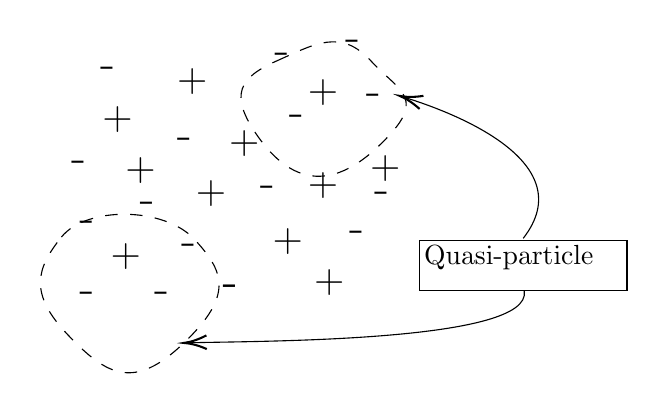
\begin{tikzpicture}[x=0.75pt,y=0.75pt,yscale=-1,xscale=1]
%uncomment if require: \path (0,300); %set diagram left start at 0, and has height of 300

%Shape: Polygon Curved [id:ds393267198766974] 
\draw  [dash pattern={on 4.5pt off 4.5pt}] (104.52,151.27) .. controls (116.52,136.27) and (154.03,136.65) .. (168.52,152.27) .. controls (183,167.88) and (187.52,179.27) .. (163.52,202.27) .. controls (139.52,225.27) and (126.52,218.27) .. (107.52,198.27) .. controls (88.52,178.27) and (92.52,166.27) .. (104.52,151.27) -- cycle ;
%Shape: Polygon Curved [id:ds5938648082047331] 
\draw  [dash pattern={on 4.5pt off 4.5pt}] (208.52,66.27) .. controls (226.52,58.27) and (239.03,50.65) .. (253.52,66.27) .. controls (268,81.88) and (281.52,84.27) .. (257.52,107.27) .. controls (233.52,130.27) and (214.52,124.27) .. (199.52,103.27) .. controls (184.52,82.27) and (190.52,74.27) .. (208.52,66.27) -- cycle ;
%Curve Lines [id:da7350178540870457] 
\draw    (327,151.88) .. controls (354.95,116) and (296.92,92.23) .. (269.18,83.77) ;
\draw [shift={(267.52,83.27)}, rotate = 376.5] [color={rgb, 255:red, 0; green, 0; blue, 0 }  ][line width=0.75]    (10.93,-3.29) .. controls (6.95,-1.4) and (3.31,-0.3) .. (0,0) .. controls (3.31,0.3) and (6.95,1.4) .. (10.93,3.29)   ;
%Curve Lines [id:da8754807282204362] 
\draw    (327.52,177.27) .. controls (331.46,201.89) and (200.54,201.29) .. (165.07,202.22) ;
\draw [shift={(163.52,202.27)}, rotate = 358.26] [color={rgb, 255:red, 0; green, 0; blue, 0 }  ][line width=0.75]    (10.93,-3.29) .. controls (6.95,-1.4) and (3.31,-0.3) .. (0,0) .. controls (3.31,0.3) and (6.95,1.4) .. (10.93,3.29)   ;

% Text Node
\draw (127,152.88) node [anchor=north west][inner sep=0.75pt]  [font=\Large] [align=left] {+};
% Text Node
\draw (141,128.88) node [anchor=north west][inner sep=0.75pt]  [font=\LARGE] [align=left] {\mbox{-}};
% Text Node
\draw (161,148.88) node [anchor=north west][inner sep=0.75pt]  [font=\LARGE] [align=left] {\mbox{-}};
% Text Node
\draw (148,171.88) node [anchor=north west][inner sep=0.75pt]  [font=\LARGE] [align=left] {\mbox{-}};
% Text Node
\draw (112,171.88) node [anchor=north west][inner sep=0.75pt]  [font=\LARGE] [align=left] {\mbox{-}};
% Text Node
\draw (112,137.88) node [anchor=north west][inner sep=0.75pt]  [font=\LARGE] [align=left] {\mbox{-}};
% Text Node
\draw (168,122.88) node [anchor=north west][inner sep=0.75pt]  [font=\Large] [align=left] {+};
% Text Node
\draw (205,145.88) node [anchor=north west][inner sep=0.75pt]  [font=\Large] [align=left] {+};
% Text Node
\draw (181,168.88) node [anchor=north west][inner sep=0.75pt]  [font=\LARGE] [align=left] {\mbox{-}};
% Text Node
\draw (181,168.88) node [anchor=north west][inner sep=0.75pt]  [font=\LARGE] [align=left] {\mbox{-}};
% Text Node
\draw (242,142.88) node [anchor=north west][inner sep=0.75pt]  [font=\LARGE] [align=left] {\mbox{-}};
% Text Node
\draw (199,120.88) node [anchor=north west][inner sep=0.75pt]  [font=\LARGE] [align=left] {\mbox{-}};
% Text Node
\draw (222,118.88) node [anchor=north west][inner sep=0.75pt]  [font=\Large] [align=left] {+};
% Text Node
\draw (184,98.88) node [anchor=north west][inner sep=0.75pt]  [font=\Large] [align=left] {+};
% Text Node
\draw (159,97.88) node [anchor=north west][inner sep=0.75pt]  [font=\LARGE] [align=left] {\mbox{-}};
% Text Node
\draw (254,123.88) node [anchor=north west][inner sep=0.75pt]  [font=\LARGE] [align=left] {\mbox{-}};
% Text Node
\draw (213,86.88) node [anchor=north west][inner sep=0.75pt]  [font=\LARGE] [align=left] {\mbox{-}};
% Text Node
\draw (250,76.88) node [anchor=north west][inner sep=0.75pt]  [font=\LARGE] [align=left] {\mbox{-}};
% Text Node
\draw (206,56.88) node [anchor=north west][inner sep=0.75pt]  [font=\LARGE] [align=left] {\mbox{-}};
% Text Node
\draw (240,50.88) node [anchor=north west][inner sep=0.75pt]  [font=\LARGE] [align=left] {\mbox{-}};
% Text Node
\draw (252,110.88) node [anchor=north west][inner sep=0.75pt]  [font=\Large] [align=left] {+};
% Text Node
\draw (222,73.88) node [anchor=north west][inner sep=0.75pt]  [font=\Large] [align=left] {+};
% Text Node
\draw (225,165.88) node [anchor=north west][inner sep=0.75pt]  [font=\Large] [align=left] {+};
% Text Node
\draw (159,68.88) node [anchor=north west][inner sep=0.75pt]  [font=\Large] [align=left] {+};
% Text Node
\draw (123,86.88) node [anchor=north west][inner sep=0.75pt]  [font=\Large] [align=left] {+};
% Text Node
\draw (108,108.88) node [anchor=north west][inner sep=0.75pt]  [font=\LARGE] [align=left] {\mbox{-}};
% Text Node
\draw (122,63.88) node [anchor=north west][inner sep=0.75pt]  [font=\LARGE] [align=left] {\mbox{-}};
% Text Node
\draw (134,111.88) node [anchor=north west][inner sep=0.75pt]  [font=\Large] [align=left] {+};
% Text Node
\draw    (277,152.88) -- (377,152.88) -- (377,176.88) -- (277,176.88) -- cycle  ;
\draw (278,153.88) node [anchor=north west][inner sep=0.75pt]   [align=left] {Quasi-particle};


\end{tikzpicture}

    \caption{Quasi particles in a Liquid of Positive and Negative Ions}
    \label{fig:quasi-particle-example}
\end{figure}
From Fig.\ref{fig:quasi-particle-example}, we know, from more powerful terminology of QFT:
\begin{center}
    "bare" particle + "clothing"/"cloud" = "dressed"/"renormalized" particle
\end{center}
For example, in quantum electrodynamics a 'bare' electron interacting with a field of photons acquires a cloud of virtual photons around it, converting it into the 'dressed' electron. In a similar manner, the interaction between real particles is called the 'bare' interaction, while the weak interaction between quasi particles is referred to as the 'effective' or "dressed" or "renormalized" interaction. \bluep{It should be noted that each bare particle is simultaneously the 'core' of a quasi particle and a transient 'member' of the cloud of several other quasi particles.}

The free quasi particles have a new energy law as 
$$\epsilon^{\prime}=\frac{p^{2}}{2 m^{*}} \quad \text { instead of } \quad \epsilon=\frac{p^{2}}{2 m}$$
where $m^*$ is the effective mass. The difference 
$$\epsilon_{quasi}-\epsilon_{bare}=\epsilon_{self}$$
is called \redp{\textbf{"self-energy"}} of the quasi particle.

@ Quantum System: quasi electreon in electron gas

The ' electron gas' is a simple model often used to describe many-body effects in metals. It consists of a box containing a large number of electrons interacting by means of the Coulomb force. In addition, there is a uniform, fixed, positive charge 'background' put into the box in order to keep the whole system electrically neutral. In the ground state, the electrons are spread out uniformly in the box.

Suppose now that we have a single, well-localized electron which we shoot into the electron gas  Because of the repulsive Coulomb interaction
between electrons, this extra electron repels other electrons away from it, so we get an empty space near the extra electron, and repelled electrons further away(Fig.\ref{fig:quasi-particle-example2}). This empty region may be viewed in a more detailed or microscopic way as composed of \redp{'holes'} in the electron gas. That is, the extra electron has "lifted out" electrons from the uniform charge distribution in its vicinity, thus creating 'holes' in this charge distribution, and has 'put down' these lifted-out electrons further away.
\begin{figure}[H]
    \centering
\tikzset {_0o14ioo3g/.code = {\pgfsetadditionalshadetransform{ \pgftransformshift{\pgfpoint{0 bp } { 0 bp }  }  \pgftransformscale{1 }  }}}
\pgfdeclareradialshading{_73ww2zakf}{\pgfpoint{0bp}{0bp}}{rgb(0bp)=(1,1,1);
rgb(12.019342694963727bp)=(1,1,1);
rgb(25bp)=(0,0,0);
rgb(400bp)=(0,0,0)}
\tikzset{_98ggw9slw/.code = {\pgfsetadditionalshadetransform{\pgftransformshift{\pgfpoint{0 bp } { 0 bp }  }  \pgftransformscale{1 } }}}
\pgfdeclareradialshading{_52d0oeat9} { \pgfpoint{0bp} {0bp}} {color(0bp)=(transparent!0);
color(12.019342694963727bp)=(transparent!0);
color(25bp)=(transparent!10);
color(400bp)=(transparent!10)} 
\pgfdeclarefading{_yzsmf2mqd}{\tikz \fill[shading=_52d0oeat9,_98ggw9slw] (0,0) rectangle (50bp,50bp); } 
\tikzset{every picture/.style={line width=0.75pt}} %set default line width to 0.75pt        

\begin{tikzpicture}[x=0.75pt,y=0.75pt,yscale=-1,xscale=1]
%uncomment if require: \path (0,300); %set diagram left start at 0, and has height of 300

%Shape: Rectangle [id:dp842398765103643] 
\draw  [fill={rgb, 255:red, 0; green, 0; blue, 0 }  ,fill opacity=1 ] (59.93,58.88) -- (235.32,58.88) -- (235.32,203.27) -- (59.93,203.27) -- cycle ;
%Shape: Circle [id:dp5878809314291961] 
\path  [shading=_73ww2zakf,_0o14ioo3g,path fading= _yzsmf2mqd ,fading transform={xshift=2}] (85.93,145.54) .. controls (85.93,131.37) and (97.42,119.88) .. (111.59,119.88) .. controls (125.76,119.88) and (137.25,131.37) .. (137.25,145.54) .. controls (137.25,159.71) and (125.76,171.2) .. (111.59,171.2) .. controls (97.42,171.2) and (85.93,159.71) .. (85.93,145.54) -- cycle ; % for fading 
 \draw   (85.93,145.54) .. controls (85.93,131.37) and (97.42,119.88) .. (111.59,119.88) .. controls (125.76,119.88) and (137.25,131.37) .. (137.25,145.54) .. controls (137.25,159.71) and (125.76,171.2) .. (111.59,171.2) .. controls (97.42,171.2) and (85.93,159.71) .. (85.93,145.54) -- cycle ; % for border 

%Shape: Circle [id:dp649192880176533] 
\draw  [fill={rgb, 255:red, 0; green, 0; blue, 0 }  ,fill opacity=1 ] (104.47,145.54) .. controls (104.47,141.61) and (107.66,138.42) .. (111.59,138.42) .. controls (115.53,138.42) and (118.72,141.61) .. (118.72,145.54) .. controls (118.72,149.48) and (115.53,152.67) .. (111.59,152.67) .. controls (107.66,152.67) and (104.47,149.48) .. (104.47,145.54) -- cycle ;
%Straight Lines [id:da47546531201986364] 
\draw [color={rgb, 255:red, 232; green, 30; blue, 12 }  ,draw opacity=1 ][line width=1.5]    (111.59,145.54) -- (135.11,122.37) ;
\draw [shift={(137.25,120.27)}, rotate = 495.43] [color={rgb, 255:red, 232; green, 30; blue, 12 }  ,draw opacity=1 ][line width=1.5]    (14.21,-4.28) .. controls (9.04,-1.82) and (4.3,-0.39) .. (0,0) .. controls (4.3,0.39) and (9.04,1.82) .. (14.21,4.28)   ;
%Shape: Rectangle [id:dp08609024153608191] 
\draw  [fill={rgb, 255:red, 0; green, 0; blue, 0 }  ,fill opacity=1 ] (261.93,58.88) -- (437.32,58.88) -- (437.32,203.27) -- (261.93,203.27) -- cycle ;
%Shape: Circle [id:dp8820237303823028] 
\draw  [fill={rgb, 255:red, 255; green, 255; blue, 255 }  ,fill opacity=1 ] (291,140.51) .. controls (291,136.3) and (294.41,132.88) .. (298.63,132.88) .. controls (302.84,132.88) and (306.25,136.3) .. (306.25,140.51) .. controls (306.25,144.72) and (302.84,148.13) .. (298.63,148.13) .. controls (294.41,148.13) and (291,144.72) .. (291,140.51) -- cycle ;
%Shape: Circle [id:dp5770389827427272] 
\draw  [fill={rgb, 255:red, 255; green, 255; blue, 255 }  ,fill opacity=1 ] (307,152.51) .. controls (307,148.3) and (310.41,144.88) .. (314.63,144.88) .. controls (318.84,144.88) and (322.25,148.3) .. (322.25,152.51) .. controls (322.25,156.72) and (318.84,160.13) .. (314.63,160.13) .. controls (310.41,160.13) and (307,156.72) .. (307,152.51) -- cycle ;
%Shape: Circle [id:dp025362450260817182] 
\draw  [fill={rgb, 255:red, 255; green, 255; blue, 255 }  ,fill opacity=1 ] (297,168.51) .. controls (297,164.3) and (300.41,160.88) .. (304.63,160.88) .. controls (308.84,160.88) and (312.25,164.3) .. (312.25,168.51) .. controls (312.25,172.72) and (308.84,176.13) .. (304.63,176.13) .. controls (300.41,176.13) and (297,172.72) .. (297,168.51) -- cycle ;
%Shape: Circle [id:dp9389847020012084] 
\draw  [fill={rgb, 255:red, 255; green, 255; blue, 255 }  ,fill opacity=1 ] (281,158.51) .. controls (281,154.3) and (284.41,150.88) .. (288.63,150.88) .. controls (292.84,150.88) and (296.25,154.3) .. (296.25,158.51) .. controls (296.25,162.72) and (292.84,166.13) .. (288.63,166.13) .. controls (284.41,166.13) and (281,162.72) .. (281,158.51) -- cycle ;
%Straight Lines [id:da4209538731972077] 
\draw [color={rgb, 255:red, 232; green, 30; blue, 12 }  ,draw opacity=1 ][line width=1.5]    (298.63,140.51) -- (293.85,117.21) ;
\draw [shift={(293.25,114.27)}, rotate = 438.42] [color={rgb, 255:red, 232; green, 30; blue, 12 }  ,draw opacity=1 ][line width=1.5]    (14.21,-4.28) .. controls (9.04,-1.82) and (4.3,-0.39) .. (0,0) .. controls (4.3,0.39) and (9.04,1.82) .. (14.21,4.28)   ;
%Straight Lines [id:da6368743975733171] 
\draw [color={rgb, 255:red, 232; green, 30; blue, 12 }  ,draw opacity=1 ][line width=1.5]    (314.63,152.51) -- (338.31,147.85) ;
\draw [shift={(341.25,147.27)}, rotate = 528.86] [color={rgb, 255:red, 232; green, 30; blue, 12 }  ,draw opacity=1 ][line width=1.5]    (14.21,-4.28) .. controls (9.04,-1.82) and (4.3,-0.39) .. (0,0) .. controls (4.3,0.39) and (9.04,1.82) .. (14.21,4.28)   ;
%Straight Lines [id:da3789740110796589] 
\draw [color={rgb, 255:red, 232; green, 30; blue, 12 }  ,draw opacity=1 ][line width=1.5]    (304.63,168.51) -- (322.7,179.69) ;
\draw [shift={(325.25,181.27)}, rotate = 211.74] [color={rgb, 255:red, 232; green, 30; blue, 12 }  ,draw opacity=1 ][line width=1.5]    (14.21,-4.28) .. controls (9.04,-1.82) and (4.3,-0.39) .. (0,0) .. controls (4.3,0.39) and (9.04,1.82) .. (14.21,4.28)   ;
%Straight Lines [id:da1630717526737726] 
\draw [color={rgb, 255:red, 232; green, 30; blue, 12 }  ,draw opacity=1 ][line width=1.5]    (288.63,158.51) -- (272.53,172.31) ;
\draw [shift={(270.25,174.27)}, rotate = 319.38] [color={rgb, 255:red, 232; green, 30; blue, 12 }  ,draw opacity=1 ][line width=1.5]    (14.21,-4.28) .. controls (9.04,-1.82) and (4.3,-0.39) .. (0,0) .. controls (4.3,0.39) and (9.04,1.82) .. (14.21,4.28)   ;

% Text Node
\draw (256,212.88) node [anchor=north west][inner sep=0.75pt]  [font=\footnotesize] [align=left] {(b)Lifted-out electrons create "holes"};
% Text Node
\draw (36,212.88) node [anchor=north west][inner sep=0.75pt]  [font=\footnotesize] [align=left] {(a)"Empty" region near the electron};


\end{tikzpicture}
    \caption{Extra Electron Pushes Other Electrons Away}
    \label{fig:quasi-particle-example2}
\end{figure}

@ Bogoliubov quasi particles ("bogolons")

These are the elementary excitations in a superconductor. We include them here since they are called quasi particles, but actually their structure is quite different from the 'particle plus cloud' picture described above. They consist of a linear combination ofan electron in state $(+k, \uparrow)$ and a hole $^{\prime}$ in $(-k, \downarrow)$.

\end{easylist}

\subsection{A Brief Intro to Collective Excitations}
As we have seen, the quasi particle consists of the original real, individual particle, plus a cloud of disturbed neighbours. It behaves very much like an
individual particle, except that it has an effective mass and a lifetime. But there also exist other kinds of fictitious particles in many-body systems, i.e., 'collective excitations'. These do not centre around individual particles, but instead involve collective, wavelike motion of all the particles in the system
simultaneously. Here are some examples:
\begin{easylist}
\NewList
@ Plasmons

If a thin metal foil is bombarded with high energy electrons, it is possible to set up sinusoidal oscillations in the density of the electron gas in the foil. This is known as a \bluep{'plasma wave'}, and it has a frequency $\omega_p$ and wavelength $\lambda_p$. \bluep{The plasma wave may be visualized as built up of 'holes' in the low-density regions and extra electrons in the high-density regions}. Just as light waves are quantized into units having energy $E=\hbar \omega$ called photons, plasma waves are quantized into units with energy $E_{p}=\hbar \omega_{p}$ called plasmons.

@ phonons

Sound waves are sinusoidal oscillations in the crystal lattice ofa solid. They are quantized into collective excitations called 'phonons'.

@ Magnons

In ferromagnets there are regular fluctuations in the density of spin angular momentum known as spin waves. The collective excitation here is the spin
wave quantum known as the 'magnon".
\end{easylist}

\subsection{Propagators-the Keys to the Many-body Problem}
The idea behind the propagator method is this: the detailed description of a many-body system requires in the classical case the position of each particle as a function of time, or in the quantum case, the time dependent wave function of the whole system. Fortunately, it turns out that \textbf{in order to find the important physical properties of a system it is not necessary to know the detailed behaviour of each particle in the system, but rather just the average behaviour of one or two typical particles.} \bluep{The quantities which describe this average behaviour are the\textit{ one-particle propagator} and \textit{two-particle propagator} respectively, and physical properties may be calculated directly from them.}

\begin{imp}
\textbf{One-particle propagator}: we put a particle into the interacting system at point $r_{1}$ at time $t_{1}$ and let it move through the system colliding with the other particles for a while (i.e., let it "propagate" through the system). Then the one-particle propagator is the probability (or in quantum systems, the probability amplitude) that the particle will be observed at the point $r_{2}$ at time $t_{2} .$ (Note that instead of putting the particle in at a definite point, it is sometimes more convenient to put it in with definite momentum, say $p_{1},$ and observe it later with momentum $p_{2} .$ ) \bluep{The single-particle propagator yields directly the energies and lifetimes of quasi particles. It also gives the momentum distribution, spin and particle density and can be used to calculate the ground state energy.}
\end{imp}
\begin{imp}
\textbf{Two-particle propagator}: the probability amplitude for observing one particle at $r_{2}, t_{2}$ and another at $r_{4}, t_{4}$ if one was put into the system at $r_{1}, t_{1}$ and another at $r_{3}, t_{3}$. This also has a wide variety of talents, \bluep{giving directly the energies and lifetimes of collective excitations, as well as the magnetic susceptibility, electrical conductivity, and a host of other non-cquilibrium properties.}
\end{imp}

\subsection{Calculate Propagator:the drunk man example}
With the aid of Feynman diagrams, we expand the propagator in an infinite series and evaluate the series approximately. This can be carried out in a general, systematic, and picturesque way.

Just to get an idea of what these diagrams are, consider the following simple example. A man who has had too much to drink, leaves a party at point 1 and on the way to his home at point 2, he can stop off at one or more bars-Alice's Bar (A), Bardot Bar (B), Club Six Bar (C), ... , etc. He can wind up either at his own home 2, or at any one of his friends' apartments, 3, 4, etc. We ask for the probability, P(2, I), that he gets home. This probability, which is just the propagator here (with time omitted for simplicity), is the sum of the probabilities for all the different ways he can propagate from I to 2 interacting with the various bars.

The first way he can prophgate is ' freely' from 1 to 2, i.e., without stopping at a bar. Call the probability for this free propagation $P_{0}(2,1)$

The second way he can propagate is to go freely from 1 to bar $A$ (the probability for this is $P_{0}(A, 1)$ ), then stop off at bar $A$ for a drink (call the probability for this $P(A))$, then go freely from $A$ to 2 (probability $=P_{0}(2, A)$ ). Assume for simplicity that the three processes here are independent. Then the total probability for this second way is the product of the probabilities for each process taken separately, i.e., $P_{0}(A, 1) \times P(A) \times P_{0}(2, A) .$ (This is like the case in coin-tossing: since each toss is independent, the probability of first tossing a head, then a tail, equals the probability of tossing a head times the probability of tossing a tail.)

The third way he can propagate is from 1 to $B$ to $2,$ with probability $P_{0}(B, 1) P(B) P_{0}(2, B) .$ Or he could go from 1 to $C$ to $2,$ etc., or from 1 to $A$ to $B$ to $2,$ or from 1 to $A,$ come out of $A,$ go back into $A,$ then go to $2,$ and so on. The total probability, $P(2,1)$ is then given by the sum of the probabilities for each way, i.e., the infinite series:
$$\begin{aligned}
P(2,1)=&P_{0}(2,1)+P_{0}(A, 1) P(A) P_{0}(2, A)+P_{0}(B, 1) P(B) P_{0}(2, B)+\cdots  \\
&+P_{0}(A, 1) P(A) P_{0}(B, A) P(B) P_{0}(2, B)+\cdots
\end{aligned}$$
\redp{This is an example of a 'perturbation series', since each interaction with a bar "perturbs" the free propagation of the drunken man.} Represent this series using the following dictionary:
\begin{figure}[H]
    \centering
\tikzset{every picture/.style={line width=0.75pt}} %set default line width to 0.75pt        

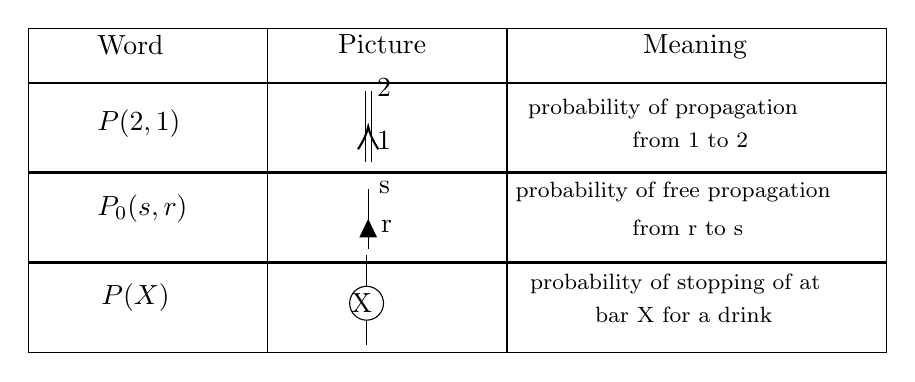
\begin{tikzpicture}[x=0.75pt,y=0.75pt,yscale=-1,xscale=1]
%uncomment if require: \path (0,349); %set diagram left start at 0, and has height of 349

%Shape: Rectangle [id:dp3972753239553969] 
\draw   (212.78,159.32) -- (328.11,159.32) -- (328.11,185.7) -- (212.78,185.7) -- cycle ;
%Shape: Rectangle [id:dp013530620031451002] 
\draw   (328.11,159.32) -- (443.44,159.32) -- (443.44,185.7) -- (328.11,185.7) -- cycle ;
%Shape: Rectangle [id:dp736076383888415] 
\draw   (443.44,159.32) -- (626.17,159.32) -- (626.17,185.7) -- (443.44,185.7) -- cycle ;
%Shape: Rectangle [id:dp018483080609867475] 
\draw   (212.78,185.32) -- (328.11,185.32) -- (328.11,229.2) -- (212.78,229.2) -- cycle ;
%Shape: Rectangle [id:dp18336509171990412] 
\draw   (328.11,185.32) -- (443.44,185.32) -- (443.44,229.2) -- (328.11,229.2) -- cycle ;
%Shape: Rectangle [id:dp5452879627568872] 
\draw   (443.44,185.32) -- (626.17,185.32) -- (626.17,229.2) -- (443.44,229.2) -- cycle ;
%Shape: Rectangle [id:dp710141061414926] 
\draw   (212.78,228.57) -- (328.11,228.57) -- (328.11,272.45) -- (212.78,272.45) -- cycle ;
%Shape: Rectangle [id:dp6981715844716105] 
\draw   (328.11,228.57) -- (443.44,228.57) -- (443.44,272.45) -- (328.11,272.45) -- cycle ;
%Shape: Rectangle [id:dp9707206740138988] 
\draw   (443.44,228.57) -- (626.17,228.57) -- (626.17,272.45) -- (443.44,272.45) -- cycle ;
%Shape: Rectangle [id:dp7188406169431831] 
\draw   (212.78,271.81) -- (328.11,271.81) -- (328.11,315.7) -- (212.78,315.7) -- cycle ;
%Shape: Rectangle [id:dp35373677352561617] 
\draw   (328.11,271.81) -- (443.44,271.81) -- (443.44,315.7) -- (328.11,315.7) -- cycle ;
%Shape: Rectangle [id:dp7761518007990666] 
\draw   (443.44,271.81) -- (626.17,271.81) -- (626.17,315.7) -- (443.44,315.7) -- cycle ;
%Straight Lines [id:da3953067075421305] 
\draw    (375.07,223.7) -- (375.07,189.7)(378.07,223.7) -- (378.07,189.7) ;
\draw [shift={(376.57,206.7)}, rotate = 450] [color={rgb, 255:red, 0; green, 0; blue, 0 }  ][line width=0.75]    (10.93,-4.9) .. controls (6.95,-2.3) and (3.31,-0.67) .. (0,0) .. controls (3.31,0.67) and (6.95,2.3) .. (10.93,4.9)   ;
%Straight Lines [id:da5701847229817978] 
\draw    (376.57,265.7) -- (376.57,236.7) ;
\draw [shift={(376.57,251.2)}, rotate = 450] [fill={rgb, 255:red, 0; green, 0; blue, 0 }  ][line width=0.08]  [draw opacity=0] (8.93,-4.29) -- (0,0) -- (8.93,4.29) -- cycle    ;
%Shape: Ellipse [id:dp16063069982491784] 
\draw   (367.64,291.82) .. controls (367.64,287.31) and (371.29,283.66) .. (375.79,283.66) .. controls (380.3,283.66) and (383.95,287.31) .. (383.95,291.82) .. controls (383.95,296.32) and (380.3,299.97) .. (375.79,299.97) .. controls (371.29,299.97) and (367.64,296.32) .. (367.64,291.82) -- cycle ;
%Straight Lines [id:da2549697012881261] 
\draw    (375.79,283.66) -- (375.79,268.7) ;
%Straight Lines [id:da05824951890975272] 
\draw    (375.79,311.7) -- (375.79,299.97) ;

% Text Node
\draw (244.78,161.32) node [anchor=north west][inner sep=0.75pt]   [align=left] {Word};
% Text Node
\draw (360.78,161.32) node [anchor=north west][inner sep=0.75pt]   [align=left] {Picture};
% Text Node
\draw (507.78,161.32) node [anchor=north west][inner sep=0.75pt]   [align=left] {Meaning};
% Text Node
\draw (244.78,197.32) node [anchor=north west][inner sep=0.75pt]    {$P( 2,1)$};
% Text Node
\draw (379.57,207.76) node [anchor=north west][inner sep=0.75pt]   [align=left] {1};
% Text Node
\draw (379.57,182.54) node [anchor=north west][inner sep=0.75pt]   [align=left] {2};
% Text Node
\draw (244.78,238.32) node [anchor=north west][inner sep=0.75pt]    {$P_{0}( s,r)$};
% Text Node
\draw (381.57,250.76) node [anchor=north west][inner sep=0.75pt]   [align=left] {r};
% Text Node
\draw (380.57,231.7) node [anchor=north west][inner sep=0.75pt]   [align=left] {s};
% Text Node
\draw (367.2,285.75) node [anchor=north west][inner sep=0.75pt]   [align=left] {X};
% Text Node
\draw (246.78,281.32) node [anchor=north west][inner sep=0.75pt]    {$P( X)$};
% Text Node
\draw (452.33,192.32) node [anchor=north west][inner sep=0.75pt]  [font=\footnotesize] [align=left] {probability of propagation };
% Text Node
\draw (502.63,208.32) node [anchor=north west][inner sep=0.75pt]  [font=\footnotesize] [align=left] {from 1 to 2};
% Text Node
\draw (446.33,232.32) node [anchor=north west][inner sep=0.75pt]  [font=\footnotesize] [align=left] {probability of free propagation };
% Text Node
\draw (502.63,250.32) node [anchor=north west][inner sep=0.75pt]  [font=\footnotesize] [align=left] {from r to s};
% Text Node
\draw (453.33,276.32) node [anchor=north west][inner sep=0.75pt]  [font=\footnotesize] [align=left] {probability of stopping of at \ };
% Text Node
\draw (484.63,292.32) node [anchor=north west][inner sep=0.75pt]  [font=\footnotesize] [align=left] {bar X for a drink};


\end{tikzpicture}

    \caption{Diagram dictionary for drunken man}
    \label{fig:drunken-man-1}
\end{figure}
The perturbation series in diagrams for this drunken man propagator is therefore
\begin{figure}[H]
    \centering
    


\tikzset{every picture/.style={line width=0.75pt}} %set default line width to 0.75pt        

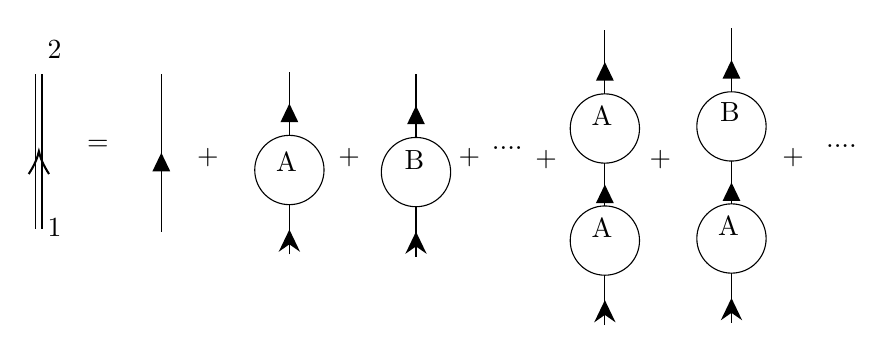
\begin{tikzpicture}[x=0.75pt,y=0.75pt,yscale=-1,xscale=1]
%uncomment if require: \path (0,349); %set diagram left start at 0, and has height of 349

%Straight Lines [id:da4757935872975344] 
\draw    (8.07,101.32) -- (8.07,26.7)(11.07,101.32) -- (11.07,26.7) ;
\draw [shift={(9.57,64.01)}, rotate = 450] [color={rgb, 255:red, 0; green, 0; blue, 0 }  ][line width=0.75]    (10.93,-4.9) .. controls (6.95,-2.3) and (3.31,-0.67) .. (0,0) .. controls (3.31,0.67) and (6.95,2.3) .. (10.93,4.9)   ;
%Straight Lines [id:da23622371172830803] 
\draw    (68.57,102.7) -- (68.57,26.7) ;
\draw [shift={(68.57,64.7)}, rotate = 450] [fill={rgb, 255:red, 0; green, 0; blue, 0 }  ][line width=0.08]  [draw opacity=0] (8.93,-4.29) -- (0,0) -- (8.93,4.29) -- cycle    ;
%Shape: Circle [id:dp4139523862436749] 
\draw   (113.57,73.01) .. controls (113.57,63.79) and (121.04,56.32) .. (130.26,56.32) .. controls (139.48,56.32) and (146.95,63.79) .. (146.95,73.01) .. controls (146.95,82.23) and (139.48,89.7) .. (130.26,89.7) .. controls (121.04,89.7) and (113.57,82.23) .. (113.57,73.01) -- cycle ;
%Straight Lines [id:da33169967910609544] 
\draw    (130.26,56.32) -- (130.26,25.7) ;
\draw [shift={(130.26,41.01)}, rotate = 450] [fill={rgb, 255:red, 0; green, 0; blue, 0 }  ][line width=0.08]  [draw opacity=0] (8.93,-4.29) -- (0,0) -- (8.93,4.29) -- cycle    ;
%Straight Lines [id:da28347419222198567] 
\draw    (130.26,113.7) -- (130.26,89.7) ;
\draw [shift={(130.26,101.7)}, rotate = 450] [fill={rgb, 255:red, 0; green, 0; blue, 0 }  ][line width=0.08]  [draw opacity=0] (10.72,-5.15) -- (0,0) -- (10.72,5.15) -- (7.12,0) -- cycle    ;
%Shape: Circle [id:dp1723289826034129] 
\draw   (174.57,74.01) .. controls (174.57,64.79) and (182.04,57.32) .. (191.26,57.32) .. controls (200.48,57.32) and (207.95,64.79) .. (207.95,74.01) .. controls (207.95,83.23) and (200.48,90.7) .. (191.26,90.7) .. controls (182.04,90.7) and (174.57,83.23) .. (174.57,74.01) -- cycle ;
%Straight Lines [id:da40381754331686626] 
\draw    (191.26,57.32) -- (191.26,26.7) ;
\draw [shift={(191.26,42.01)}, rotate = 450] [fill={rgb, 255:red, 0; green, 0; blue, 0 }  ][line width=0.08]  [draw opacity=0] (8.93,-4.29) -- (0,0) -- (8.93,4.29) -- cycle    ;
%Straight Lines [id:da5172106067784763] 
\draw    (191.26,114.7) -- (191.26,90.7) ;
\draw [shift={(191.26,102.7)}, rotate = 450] [fill={rgb, 255:red, 0; green, 0; blue, 0 }  ][line width=0.08]  [draw opacity=0] (10.72,-5.15) -- (0,0) -- (10.72,5.15) -- (7.12,0) -- cycle    ;
%Shape: Circle [id:dp663325870350397] 
\draw   (265.57,107.01) .. controls (265.57,97.79) and (273.04,90.32) .. (282.26,90.32) .. controls (291.48,90.32) and (298.95,97.79) .. (298.95,107.01) .. controls (298.95,116.23) and (291.48,123.7) .. (282.26,123.7) .. controls (273.04,123.7) and (265.57,116.23) .. (265.57,107.01) -- cycle ;
%Straight Lines [id:da6913773132395338] 
\draw    (282.26,36.32) -- (282.26,5.7) ;
\draw [shift={(282.26,21.01)}, rotate = 450] [fill={rgb, 255:red, 0; green, 0; blue, 0 }  ][line width=0.08]  [draw opacity=0] (8.93,-4.29) -- (0,0) -- (8.93,4.29) -- cycle    ;
%Straight Lines [id:da4724377841227787] 
\draw    (282.26,147.7) -- (282.26,123.7) ;
\draw [shift={(282.26,135.7)}, rotate = 450] [fill={rgb, 255:red, 0; green, 0; blue, 0 }  ][line width=0.08]  [draw opacity=0] (10.72,-5.15) -- (0,0) -- (10.72,5.15) -- (7.12,0) -- cycle    ;
%Shape: Circle [id:dp29262051024858293] 
\draw   (265.57,53.01) .. controls (265.57,43.79) and (273.04,36.32) .. (282.26,36.32) .. controls (291.48,36.32) and (298.95,43.79) .. (298.95,53.01) .. controls (298.95,62.23) and (291.48,69.7) .. (282.26,69.7) .. controls (273.04,69.7) and (265.57,62.23) .. (265.57,53.01) -- cycle ;
%Straight Lines [id:da2293551017015375] 
\draw    (282.26,69.7) -- (282.26,90.32) ;
\draw [shift={(282.26,80.01)}, rotate = 90] [fill={rgb, 255:red, 0; green, 0; blue, 0 }  ][line width=0.08]  [draw opacity=0] (8.93,-4.29) -- (0,0) -- (8.93,4.29) -- cycle    ;
%Shape: Circle [id:dp5742274191772756] 
\draw   (326.57,106.01) .. controls (326.57,96.79) and (334.04,89.32) .. (343.26,89.32) .. controls (352.48,89.32) and (359.95,96.79) .. (359.95,106.01) .. controls (359.95,115.23) and (352.48,122.7) .. (343.26,122.7) .. controls (334.04,122.7) and (326.57,115.23) .. (326.57,106.01) -- cycle ;
%Straight Lines [id:da8337372469854066] 
\draw    (343.26,35.32) -- (343.26,4.7) ;
\draw [shift={(343.26,20.01)}, rotate = 450] [fill={rgb, 255:red, 0; green, 0; blue, 0 }  ][line width=0.08]  [draw opacity=0] (8.93,-4.29) -- (0,0) -- (8.93,4.29) -- cycle    ;
%Straight Lines [id:da42712440571211296] 
\draw    (343.26,146.7) -- (343.26,122.7) ;
\draw [shift={(343.26,134.7)}, rotate = 450] [fill={rgb, 255:red, 0; green, 0; blue, 0 }  ][line width=0.08]  [draw opacity=0] (10.72,-5.15) -- (0,0) -- (10.72,5.15) -- (7.12,0) -- cycle    ;
%Shape: Circle [id:dp5287893719741432] 
\draw   (326.57,52.01) .. controls (326.57,42.79) and (334.04,35.32) .. (343.26,35.32) .. controls (352.48,35.32) and (359.95,42.79) .. (359.95,52.01) .. controls (359.95,61.23) and (352.48,68.7) .. (343.26,68.7) .. controls (334.04,68.7) and (326.57,61.23) .. (326.57,52.01) -- cycle ;
%Straight Lines [id:da8377025286119076] 
\draw    (343.26,68.7) -- (343.26,89.32) ;
\draw [shift={(343.26,79.01)}, rotate = 90] [fill={rgb, 255:red, 0; green, 0; blue, 0 }  ][line width=0.08]  [draw opacity=0] (8.93,-4.29) -- (0,0) -- (8.93,4.29) -- cycle    ;

% Text Node
\draw (12.57,95.32) node [anchor=north west][inner sep=0.75pt]   [align=left] {1};
% Text Node
\draw (12.57,9.32) node [anchor=north west][inner sep=0.75pt]   [align=left] {2};
% Text Node
\draw (31.57,57.32) node [anchor=north west][inner sep=0.75pt]   [align=left] {=};
% Text Node
\draw (122.57,63.32) node [anchor=north west][inner sep=0.75pt]   [align=left] {A};
% Text Node
\draw (184.57,62.32) node [anchor=north west][inner sep=0.75pt]   [align=left] {B};
% Text Node
\draw (336.57,39.32) node [anchor=north west][inner sep=0.75pt]   [align=left] {B};
% Text Node
\draw (335.57,94.32) node [anchor=north west][inner sep=0.75pt]   [align=left] {A};
% Text Node
\draw (274.57,95.32) node [anchor=north west][inner sep=0.75pt]   [align=left] {A};
% Text Node
\draw (274.57,41.32) node [anchor=north west][inner sep=0.75pt]   [align=left] {A};
% Text Node
\draw (84.57,61.32) node [anchor=north west][inner sep=0.75pt]    {$+$};
% Text Node
\draw (152.57,61.32) node [anchor=north west][inner sep=0.75pt]    {$+$};
% Text Node
\draw (210.57,61.32) node [anchor=north west][inner sep=0.75pt]    {$+$};
% Text Node
\draw (226.57,60.32) node [anchor=north west][inner sep=0.75pt]   [align=left] {....};
% Text Node
\draw (247.57,62.32) node [anchor=north west][inner sep=0.75pt]    {$+$};
% Text Node
\draw (302.57,62.32) node [anchor=north west][inner sep=0.75pt]    {$+$};
% Text Node
\draw (366.57,61.32) node [anchor=north west][inner sep=0.75pt]    {$+$};
% Text Node
\draw (387.57,59.32) node [anchor=north west][inner sep=0.75pt]   [align=left] {....};


\end{tikzpicture}

    \caption{Drunken man series}
    \label{fig:drunken-man-2}
\end{figure}

\subsection{Single-particle propagator for system of many interacting particles}
We now describe a second-order propagation process as following:
\begin{itemize}
    \item At time $t_1$, extra particle enters system
    \item At time t, extra particle interacts with a particle (through virtual photon) in the system, lifting it out of its place, creating a "hole" in the system
    \item The extra particle, plus the "hole" and the "lifted-out" particle(\redp{particle-hole pair}) travel through the system
    \item At time $t^{\prime}$, the extra particle interacts with  "lifted-out" particle, knocking it back into the hole, thus destroying the particle-hole pair.
    \item At time $t_2$, the extra particle moves out of the system.
\end{itemize}
We use the following diagram elements here.\bluep{Note that the hole is drawn as a particle moving backward in time}.
\begin{figure}[H]
    \centering
\tikzset{every picture/.style={line width=0.75pt}} %set default line width to 0.75pt        

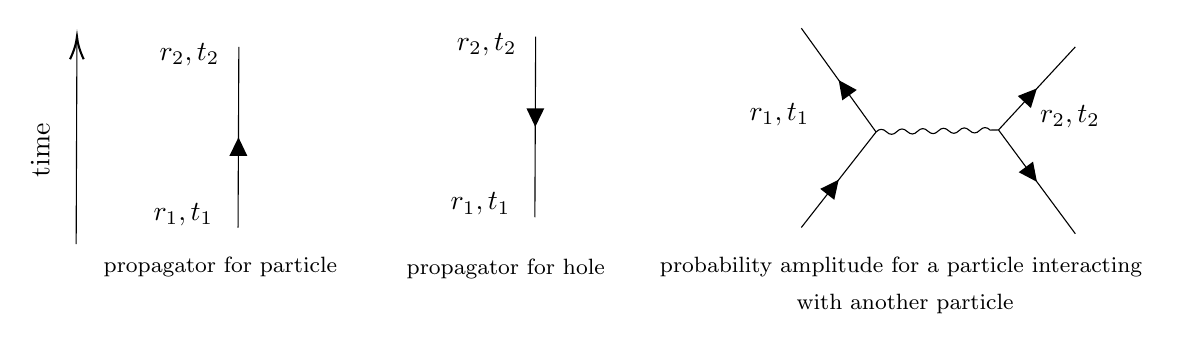
\begin{tikzpicture}[x=0.75pt,y=0.75pt,yscale=-1,xscale=1]
%uncomment if require: \path (0,300); %set diagram left start at 0, and has height of 300

%Straight Lines [id:da19133695979745402] 
\draw    (190.28,120) -- (190.67,32.93) ;
\draw [shift={(190.48,76.47)}, rotate = 450.25] [fill={rgb, 255:red, 0; green, 0; blue, 0 }  ][line width=0.08]  [draw opacity=0] (8.93,-4.29) -- (0,0) -- (8.93,4.29) -- cycle    ;
%Straight Lines [id:da8918233616398107] 
\draw    (112.28,128) -- (112.66,29.93) ;
\draw [shift={(112.67,27.93)}, rotate = 450.22] [color={rgb, 255:red, 0; green, 0; blue, 0 }  ][line width=0.75]    (10.93,-3.29) .. controls (6.95,-1.4) and (3.31,-0.3) .. (0,0) .. controls (3.31,0.3) and (6.95,1.4) .. (10.93,3.29)   ;
%Straight Lines [id:da9519966290540162] 
\draw    (333.29,115) -- (333.67,27.93) ;
\draw [shift={(333.48,71.47)}, rotate = 270.25] [fill={rgb, 255:red, 0; green, 0; blue, 0 }  ][line width=0.08]  [draw opacity=0] (8.93,-4.29) -- (0,0) -- (8.93,4.29) -- cycle    ;
%Straight Lines [id:da7312209816881998] 
\draw    (593.67,122.93) -- (556.67,72.93) ;
\draw [shift={(575.17,97.93)}, rotate = 233.5] [fill={rgb, 255:red, 0; green, 0; blue, 0 }  ][line width=0.08]  [draw opacity=0] (8.93,-4.29) -- (0,0) -- (8.93,4.29) -- cycle    ;
%Straight Lines [id:da37095749047846227] 
\draw    (593.67,32.93) -- (556.67,72.93) ;
\draw [shift={(575.17,52.93)}, rotate = 132.77] [fill={rgb, 255:red, 0; green, 0; blue, 0 }  ][line width=0.08]  [draw opacity=0] (8.93,-4.29) -- (0,0) -- (8.93,4.29) -- cycle    ;
%Straight Lines [id:da18873008311254413] 
\draw    (497.67,73.93) -- (461.67,23.93) ;
\draw [shift={(479.67,48.93)}, rotate = 414.25] [fill={rgb, 255:red, 0; green, 0; blue, 0 }  ][line width=0.08]  [draw opacity=0] (8.93,-4.29) -- (0,0) -- (8.93,4.29) -- cycle    ;
%Straight Lines [id:da6044480912830338] 
\draw    (497.67,73.93) -- (461.67,119.93) ;
\draw [shift={(479.67,96.93)}, rotate = 128.05] [fill={rgb, 255:red, 0; green, 0; blue, 0 }  ][line width=0.08]  [draw opacity=0] (8.93,-4.29) -- (0,0) -- (8.93,4.29) -- cycle    ;
%Straight Lines [id:da35473256420919863] 
\draw    (497.67,73.93) .. controls (499.31,72.24) and (500.98,72.21) .. (502.67,73.85) .. controls (504.36,75.48) and (506.03,75.45) .. (507.67,73.76) .. controls (509.3,72.07) and (510.97,72.04) .. (512.66,73.68) .. controls (514.35,75.31) and (516.02,75.28) .. (517.66,73.59) .. controls (519.3,71.9) and (520.97,71.87) .. (522.66,73.51) .. controls (524.35,75.14) and (526.02,75.11) .. (527.66,73.42) .. controls (529.3,71.73) and (530.97,71.7) .. (532.66,73.34) .. controls (534.35,74.98) and (536.02,74.95) .. (537.66,73.26) .. controls (539.3,71.57) and (540.97,71.54) .. (542.66,73.17) .. controls (544.35,74.81) and (546.02,74.78) .. (547.66,73.09) .. controls (549.3,71.4) and (550.97,71.37) .. (552.66,73) -- (556.67,72.93) -- (556.67,72.93) ;

% Text Node
\draw (89.19,96.94) node [anchor=north west][inner sep=0.75pt]  [rotate=-270.31] [align=left] {time};
% Text Node
\draw (148.28,107) node [anchor=north west][inner sep=0.75pt]    {$r_{1} ,t_{1}$};
% Text Node
\draw (151.28,30) node [anchor=north west][inner sep=0.75pt]    {$r_{2} ,t_{2}$};
% Text Node
\draw (124.28,133) node [anchor=north west][inner sep=0.75pt]  [font=\footnotesize] [align=left] {propagator for particle};
% Text Node
\draw (291.49,102) node [anchor=north west][inner sep=0.75pt]    {$r_{1} ,t_{1}$};
% Text Node
\draw (294.46,25) node [anchor=north west][inner sep=0.75pt]    {$r_{2} ,t_{2}$};
% Text Node
\draw (270.28,134) node [anchor=north west][inner sep=0.75pt]  [font=\footnotesize] [align=left] {propagator for hole};
% Text Node
\draw (435.49,59) node [anchor=north west][inner sep=0.75pt]    {$r_{1} ,t_{1}$};
% Text Node
\draw (575.46,60) node [anchor=north west][inner sep=0.75pt]    {$r_{2} ,t_{2}$};
% Text Node
\draw (392.28,133) node [anchor=north west][inner sep=0.75pt]  [font=\footnotesize] [align=left] {probability amplitude for a particle interacting };
% Text Node
\draw (458.13,151) node [anchor=north west][inner sep=0.75pt]  [font=\footnotesize] [align=left] {with another particle};


\end{tikzpicture}

    \caption{Diagram elements for second-order propagation}
    \label{fig:elem-2nd-propagator}
\end{figure}
Then the probability amplitude for the above sequence of events can be represented by the diagram
\begin{center}
\tikzset{every picture/.style={line width=0.75pt}} %set default line width to 0.75pt        

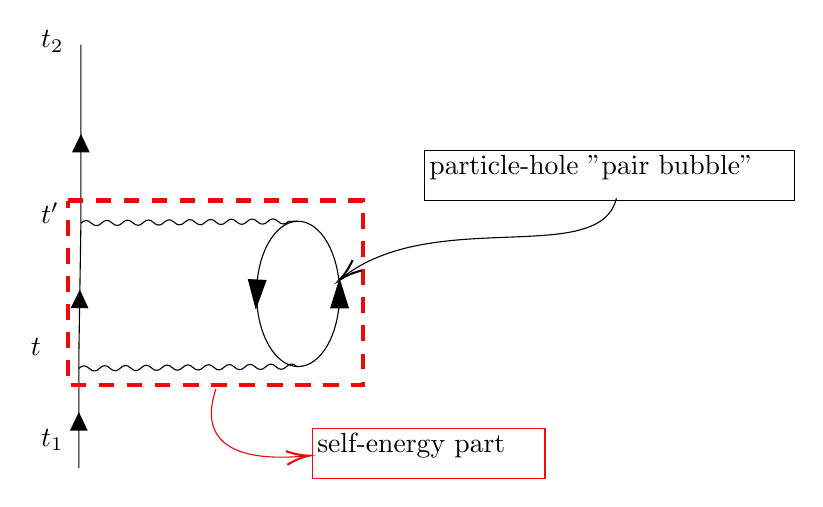
\begin{tikzpicture}[x=0.75pt,y=0.75pt,yscale=-1,xscale=1]
%uncomment if require: \path (0,300); %set diagram left start at 0, and has height of 300

%Straight Lines [id:da3914578805076815] 
\draw    (239.9,40.93) -- (239.9,126.93) -- (238.9,190.93) -- (238.9,244.93) ;
\draw [shift={(239.9,83.93)}, rotate = 90] [fill={rgb, 255:red, 0; green, 0; blue, 0 }  ][line width=0.08]  [draw opacity=0] (8.93,-4.29) -- (0,0) -- (8.93,4.29) -- cycle    ;
\draw [shift={(239.4,158.93)}, rotate = 90.9] [fill={rgb, 255:red, 0; green, 0; blue, 0 }  ][line width=0.08]  [draw opacity=0] (8.93,-4.29) -- (0,0) -- (8.93,4.29) -- cycle    ;
\draw [shift={(238.9,217.93)}, rotate = 90] [fill={rgb, 255:red, 0; green, 0; blue, 0 }  ][line width=0.08]  [draw opacity=0] (8.93,-4.29) -- (0,0) -- (8.93,4.29) -- cycle    ;
%Shape: Ellipse [id:dp4458035019540618] 
\draw   (344.57,196) .. controls (333.53,196.02) and (324.55,180.36) .. (324.52,161.03) .. controls (324.49,141.7) and (333.42,126.02) .. (344.46,126) .. controls (355.51,125.98) and (364.49,141.64) .. (364.52,160.97) .. controls (364.55,180.3) and (355.62,195.98) .. (344.57,196) -- cycle ;
%Straight Lines [id:da03751642849998316] 
\draw    (239.9,126.93) .. controls (241.55,125.25) and (243.22,125.24) .. (244.9,126.89) .. controls (246.58,128.54) and (248.25,128.52) .. (249.9,126.84) .. controls (251.55,125.16) and (253.22,125.15) .. (254.9,126.8) .. controls (256.58,128.45) and (258.25,128.43) .. (259.9,126.75) .. controls (261.55,125.07) and (263.22,125.06) .. (264.9,126.71) .. controls (266.58,128.36) and (268.25,128.35) .. (269.9,126.67) .. controls (271.55,124.99) and (273.22,124.97) .. (274.9,126.62) .. controls (276.58,128.27) and (278.25,128.26) .. (279.9,126.58) .. controls (281.55,124.9) and (283.22,124.88) .. (284.9,126.53) .. controls (286.58,128.18) and (288.25,128.17) .. (289.9,126.49) .. controls (291.55,124.81) and (293.22,124.79) .. (294.9,126.44) .. controls (296.58,128.09) and (298.25,128.08) .. (299.9,126.4) .. controls (301.55,124.72) and (303.22,124.7) .. (304.9,126.35) .. controls (306.58,128) and (308.25,127.99) .. (309.9,126.31) .. controls (311.55,124.63) and (313.22,124.61) .. (314.9,126.26) .. controls (316.58,127.91) and (318.25,127.9) .. (319.9,126.22) .. controls (321.55,124.54) and (323.22,124.52) .. (324.9,126.17) .. controls (326.58,127.82) and (328.25,127.81) .. (329.9,126.13) .. controls (331.55,124.45) and (333.22,124.44) .. (334.9,126.09) .. controls (336.58,127.74) and (338.25,127.72) .. (339.9,126.04) -- (344.46,126) -- (344.46,126) ;
%Straight Lines [id:da22386446930432802] 
\draw    (238.9,196.93) .. controls (240.55,195.25) and (242.22,195.24) .. (243.9,196.89) .. controls (245.58,198.54) and (247.25,198.53) .. (248.9,196.85) .. controls (250.55,195.17) and (252.22,195.15) .. (253.9,196.8) .. controls (255.58,198.45) and (257.25,198.44) .. (258.9,196.76) .. controls (260.55,195.08) and (262.22,195.06) .. (263.9,196.71) .. controls (265.58,198.36) and (267.25,198.35) .. (268.9,196.67) .. controls (270.55,194.99) and (272.22,194.97) .. (273.9,196.62) .. controls (275.58,198.27) and (277.25,198.26) .. (278.9,196.58) .. controls (280.55,194.9) and (282.22,194.89) .. (283.9,196.54) .. controls (285.58,198.19) and (287.25,198.17) .. (288.9,196.49) .. controls (290.55,194.81) and (292.22,194.8) .. (293.9,196.45) .. controls (295.58,198.1) and (297.25,198.08) .. (298.9,196.4) .. controls (300.55,194.72) and (302.22,194.71) .. (303.9,196.36) .. controls (305.58,198.01) and (307.25,198) .. (308.9,196.32) .. controls (310.55,194.64) and (312.22,194.62) .. (313.9,196.27) .. controls (315.58,197.92) and (317.25,197.91) .. (318.9,196.23) .. controls (320.55,194.55) and (322.22,194.53) .. (323.9,196.18) .. controls (325.58,197.83) and (327.25,197.82) .. (328.9,196.14) .. controls (330.55,194.46) and (332.22,194.44) .. (333.9,196.09) .. controls (335.58,197.74) and (337.25,197.73) .. (338.9,196.05) .. controls (340.55,194.37) and (342.22,194.36) .. (343.9,196.01) -- (344.57,196) -- (344.57,196) ;
%Shape: Triangle [id:dp8438251936972118] 
\draw  [fill={rgb, 255:red, 0; green, 0; blue, 0 }  ,fill opacity=1 ] (364.52,154.25) -- (368.71,167.68) -- (360.32,167.68) -- cycle ;
%Shape: Triangle [id:dp13261991584446953] 
\draw  [fill={rgb, 255:red, 0; green, 0; blue, 0 }  ,fill opacity=1 ] (324.2,167.74) -- (320.64,154.13) -- (329.02,154.52) -- cycle ;
%Shape: Rectangle [id:dp26500062559360993] 
\draw  [color={rgb, 255:red, 239; green, 9; blue, 9 }  ,draw opacity=1 ][dash pattern={on 5.63pt off 4.5pt}][line width=1.5]  (233.52,116) -- (375.9,116) -- (375.9,204.93) -- (233.52,204.93) -- cycle ;
%Curve Lines [id:da7889824653675461] 
\draw [color={rgb, 255:red, 233; green, 8; blue, 8 }  ,draw opacity=1 ]   (304.9,206.93) .. controls (297.02,230.57) and (310.86,242.51) .. (348.18,239.1) ;
\draw [shift={(349.9,238.93)}, rotate = 534.1800000000001] [color={rgb, 255:red, 233; green, 8; blue, 8 }  ,draw opacity=1 ][line width=0.75]    (10.93,-3.29) .. controls (6.95,-1.4) and (3.31,-0.3) .. (0,0) .. controls (3.31,0.3) and (6.95,1.4) .. (10.93,3.29)   ;
%Curve Lines [id:da8696448552998278] 
\draw    (497.9,114.93) .. controls (489.98,148.59) and (409.53,118.55) .. (365.83,153.18) ;
\draw [shift={(364.52,154.25)}, rotate = 320.06] [color={rgb, 255:red, 0; green, 0; blue, 0 }  ][line width=0.75]    (10.93,-3.29) .. controls (6.95,-1.4) and (3.31,-0.3) .. (0,0) .. controls (3.31,0.3) and (6.95,1.4) .. (10.93,3.29)   ;

% Text Node
\draw (219.52,225) node [anchor=north west][inner sep=0.75pt]    {$t_{1}$};
% Text Node
\draw (214.52,181) node [anchor=north west][inner sep=0.75pt]    {$t$};
% Text Node
\draw (219.52,116) node [anchor=north west][inner sep=0.75pt]    {$t^{\prime }$};
% Text Node
\draw (219.52,33) node [anchor=north west][inner sep=0.75pt]    {$t_{2}$};
% Text Node
\draw  [color={rgb, 255:red, 244; green, 10; blue, 10 }  ,draw opacity=1 ]  (351.52,226) -- (463.52,226) -- (463.52,250) -- (351.52,250) -- cycle  ;
\draw (352.52,227) node [anchor=north west][inner sep=0.75pt]   [align=left] {self-energy part};
% Text Node
\draw    (405.52,92) -- (583.52,92) -- (583.52,116) -- (405.52,116) -- cycle  ;
\draw (406.52,93) node [anchor=north west][inner sep=0.75pt]   [align=left] {particle-hole "pair bubble"};


\end{tikzpicture}

\end{center}
where we have a so-called "self-energy part" because it shows the particle interacting with itself via the particle-hole pair it created in the many-body medium.

Another sequence of events which can occur involves only one interaction (i.e., a 'first-order ' process). It is a \bluep{quick-change act in which the incoming electron at point r interacts with another electron at point r' and changes place with it}. This is analogous to billiard ball 1 striking billiard ball 2 and transferring all its momentum to 2. The process sequence is:
\begin{itemize}
    \item Extra particle enters at time $t_1$
    \item At time $t$, the particles is at point $r$. It interacts with a particle at $r^{\prime}$(through virtual photon) and changes place with it.
    \item Extra particle leaves at time $t_2$
\end{itemize}
with a "open oyster" diagram as below:
\begin{center}
    


\tikzset{every picture/.style={line width=0.75pt}} %set default line width to 0.75pt        

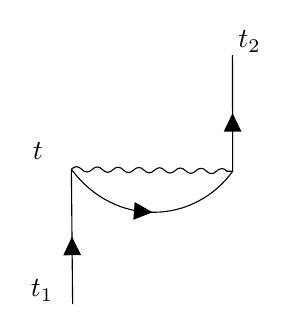
\begin{tikzpicture}[x=0.75pt,y=0.75pt,yscale=-1,xscale=1]
%uncomment if require: \path (0,300); %set diagram left start at 0, and has height of 300

%Curve Lines [id:da7645811334291478] 
\draw    (486.9,124.93) .. controls (507.62,152.93) and (545.62,151.93) .. (564.62,125.93) ;
\draw [shift={(525.97,145.68)}, rotate = 184.29] [fill={rgb, 255:red, 0; green, 0; blue, 0 }  ][line width=0.08]  [draw opacity=0] (8.93,-4.29) -- (0,0) -- (8.93,4.29) -- cycle    ;
%Straight Lines [id:da0067325630711646545] 
\draw    (486.9,124.93) -- (487.5,189.93) ;
\draw [shift={(487.2,157.43)}, rotate = 89.47] [fill={rgb, 255:red, 0; green, 0; blue, 0 }  ][line width=0.08]  [draw opacity=0] (8.93,-4.29) -- (0,0) -- (8.93,4.29) -- cycle    ;
%Straight Lines [id:da31755570766840036] 
\draw    (486.9,124.93) .. controls (488.59,123.29) and (490.25,123.31) .. (491.9,125) .. controls (493.55,126.69) and (495.21,126.71) .. (496.9,125.06) .. controls (498.59,123.42) and (500.25,123.44) .. (501.9,125.13) .. controls (503.55,126.82) and (505.21,126.84) .. (506.9,125.19) .. controls (508.59,123.54) and (510.25,123.56) .. (511.9,125.25) .. controls (513.55,126.94) and (515.21,126.96) .. (516.9,125.32) .. controls (518.59,123.67) and (520.25,123.69) .. (521.9,125.38) .. controls (523.55,127.07) and (525.21,127.09) .. (526.9,125.45) .. controls (528.59,123.8) and (530.25,123.82) .. (531.9,125.51) .. controls (533.55,127.2) and (535.21,127.22) .. (536.9,125.58) .. controls (538.59,123.93) and (540.25,123.95) .. (541.9,125.64) .. controls (543.55,127.33) and (545.21,127.35) .. (546.9,125.71) .. controls (548.59,124.06) and (550.25,124.08) .. (551.89,125.77) .. controls (553.54,127.46) and (555.2,127.48) .. (556.89,125.83) .. controls (558.58,124.19) and (560.24,124.21) .. (561.89,125.9) -- (564.62,125.93) -- (564.62,125.93) ;
%Straight Lines [id:da6864724196774904] 
\draw    (564.62,125.93) -- (564.5,69.93) ;
\draw [shift={(564.56,97.93)}, rotate = 449.88] [fill={rgb, 255:red, 0; green, 0; blue, 0 }  ][line width=0.08]  [draw opacity=0] (8.93,-4.29) -- (0,0) -- (8.93,4.29) -- cycle    ;

% Text Node
\draw (466.12,177) node [anchor=north west][inner sep=0.75pt]    {$t_{1}$};
% Text Node
\draw (566.12,57) node [anchor=north west][inner sep=0.75pt]    {$t_{2}$};
% Text Node
\draw (467.12,111) node [anchor=north west][inner sep=0.75pt]    {$t$};


\end{tikzpicture}
\end{center}

We can see the direct connection between the one-particle propagator and the quasi particle by looking at all the diagrams at a particular time $t_0$ (dashed line)
\begin{center}

\tikzset{every picture/.style={line width=0.75pt}} %set default line width to 0.75pt        

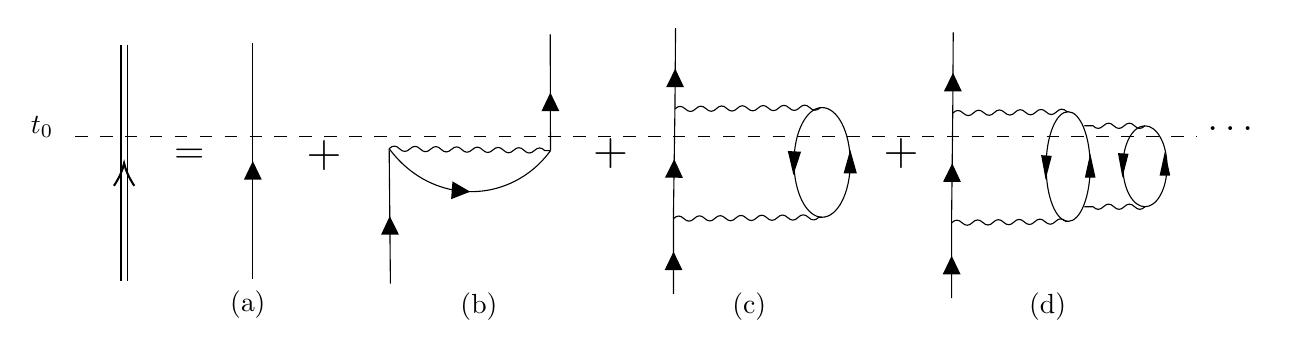
\begin{tikzpicture}[x=0.75pt,y=0.75pt,yscale=-1,xscale=1]
%uncomment if require: \path (0,300); %set diagram left start at 0, and has height of 300

%Straight Lines [id:da3914578805076815] 
\draw    (343.88,60.93) -- (343.58,99.85) -- (342.9,148.17) -- (342.9,188.93) ;
\draw [shift={(343.73,80.39)}, rotate = 90.45] [fill={rgb, 255:red, 0; green, 0; blue, 0 }  ][line width=0.08]  [draw opacity=0] (8.93,-4.29) -- (0,0) -- (8.93,4.29) -- cycle    ;
\draw [shift={(343.24,124.01)}, rotate = 90.8] [fill={rgb, 255:red, 0; green, 0; blue, 0 }  ][line width=0.08]  [draw opacity=0] (8.93,-4.29) -- (0,0) -- (8.93,4.29) -- cycle    ;
\draw [shift={(342.9,168.55)}, rotate = 90] [fill={rgb, 255:red, 0; green, 0; blue, 0 }  ][line width=0.08]  [draw opacity=0] (8.93,-4.29) -- (0,0) -- (8.93,4.29) -- cycle    ;
%Shape: Ellipse [id:dp4458035019540618] 
\draw   (414.52,151.99) .. controls (407.04,152.01) and (400.95,140.19) .. (400.93,125.6) .. controls (400.91,111) and (406.96,99.16) .. (414.45,99.15) .. controls (421.94,99.14) and (428.02,110.96) .. (428.04,125.55) .. controls (428.06,140.14) and (422.01,151.98) .. (414.52,151.99) -- cycle ;
%Straight Lines [id:da03751642849998316] 
\draw    (343.58,99.85) .. controls (345.23,98.17) and (346.9,98.16) .. (348.58,99.81) .. controls (350.26,101.46) and (351.93,101.44) .. (353.58,99.76) .. controls (355.23,98.08) and (356.9,98.06) .. (358.58,99.71) .. controls (360.26,101.36) and (361.93,101.34) .. (363.58,99.66) .. controls (365.23,97.98) and (366.9,97.96) .. (368.58,99.61) .. controls (370.26,101.26) and (371.93,101.24) .. (373.58,99.56) .. controls (375.23,97.88) and (376.9,97.86) .. (378.58,99.51) .. controls (380.26,101.16) and (381.93,101.14) .. (383.58,99.46) .. controls (385.23,97.78) and (386.9,97.76) .. (388.58,99.41) .. controls (390.26,101.06) and (391.93,101.04) .. (393.58,99.36) .. controls (395.23,97.68) and (396.9,97.66) .. (398.58,99.31) .. controls (400.26,100.96) and (401.92,100.94) .. (403.57,99.26) .. controls (405.22,97.58) and (406.89,97.56) .. (408.57,99.21) .. controls (410.25,100.86) and (411.92,100.84) .. (413.57,99.16) -- (414.45,99.15) -- (414.45,99.15) ;
%Straight Lines [id:da22386446930432802] 
\draw    (342.9,152.7) .. controls (344.55,151.01) and (346.22,151) .. (347.9,152.65) .. controls (349.58,154.3) and (351.25,154.28) .. (352.9,152.6) .. controls (354.55,150.92) and (356.22,150.9) .. (357.9,152.55) .. controls (359.58,154.2) and (361.25,154.18) .. (362.9,152.5) .. controls (364.55,150.82) and (366.22,150.8) .. (367.9,152.45) .. controls (369.58,154.1) and (371.25,154.08) .. (372.9,152.4) .. controls (374.55,150.72) and (376.22,150.7) .. (377.9,152.35) .. controls (379.58,154) and (381.25,153.98) .. (382.9,152.3) .. controls (384.55,150.62) and (386.22,150.61) .. (387.9,152.26) .. controls (389.58,153.91) and (391.25,153.89) .. (392.9,152.21) .. controls (394.55,150.53) and (396.22,150.51) .. (397.9,152.16) .. controls (399.58,153.81) and (401.25,153.79) .. (402.9,152.11) .. controls (404.55,150.43) and (406.22,150.41) .. (407.9,152.06) .. controls (409.58,153.71) and (411.25,153.69) .. (412.9,152.01) -- (414.52,151.99) -- (414.52,151.99) ;
%Shape: Triangle [id:dp8438251936972118] 
\draw  [fill={rgb, 255:red, 0; green, 0; blue, 0 }  ,fill opacity=1 ] (428.04,120.48) -- (430.88,130.62) -- (425.2,130.62) -- cycle ;
%Shape: Triangle [id:dp13261991584446953] 
\draw  [fill={rgb, 255:red, 0; green, 0; blue, 0 }  ,fill opacity=1 ] (400.72,130.66) -- (398.31,120.38) -- (403.98,120.68) -- cycle ;
%Curve Lines [id:da7645811334291478] 
\draw    (205.9,118.93) .. controls (226.62,146.93) and (264.62,145.93) .. (283.62,119.93) ;
\draw [shift={(244.97,139.68)}, rotate = 184.29] [fill={rgb, 255:red, 0; green, 0; blue, 0 }  ][line width=0.08]  [draw opacity=0] (8.93,-4.29) -- (0,0) -- (8.93,4.29) -- cycle    ;
%Straight Lines [id:da0067325630711646545] 
\draw    (205.9,118.93) -- (206.5,183.93) ;
\draw [shift={(206.2,151.43)}, rotate = 89.47] [fill={rgb, 255:red, 0; green, 0; blue, 0 }  ][line width=0.08]  [draw opacity=0] (8.93,-4.29) -- (0,0) -- (8.93,4.29) -- cycle    ;
%Straight Lines [id:da31755570766840036] 
\draw    (205.9,118.93) .. controls (207.59,117.29) and (209.25,117.31) .. (210.9,119) .. controls (212.55,120.69) and (214.21,120.71) .. (215.9,119.06) .. controls (217.59,117.42) and (219.25,117.44) .. (220.9,119.13) .. controls (222.55,120.82) and (224.21,120.84) .. (225.9,119.19) .. controls (227.59,117.54) and (229.25,117.56) .. (230.9,119.25) .. controls (232.55,120.94) and (234.21,120.96) .. (235.9,119.32) .. controls (237.59,117.67) and (239.25,117.69) .. (240.9,119.38) .. controls (242.55,121.07) and (244.21,121.09) .. (245.9,119.45) .. controls (247.59,117.8) and (249.25,117.82) .. (250.9,119.51) .. controls (252.55,121.2) and (254.21,121.22) .. (255.9,119.58) .. controls (257.59,117.93) and (259.25,117.95) .. (260.9,119.64) .. controls (262.55,121.33) and (264.21,121.35) .. (265.9,119.71) .. controls (267.59,118.06) and (269.25,118.08) .. (270.89,119.77) .. controls (272.54,121.46) and (274.2,121.48) .. (275.89,119.83) .. controls (277.58,118.19) and (279.24,118.21) .. (280.89,119.9) -- (283.62,119.93) -- (283.62,119.93) ;
%Straight Lines [id:da6864724196774904] 
\draw    (283.62,119.93) -- (283.5,63.93) ;
\draw [shift={(283.56,91.93)}, rotate = 449.88] [fill={rgb, 255:red, 0; green, 0; blue, 0 }  ][line width=0.08]  [draw opacity=0] (8.93,-4.29) -- (0,0) -- (8.93,4.29) -- cycle    ;
%Straight Lines [id:da0059350286742723135] 
\draw    (477.67,62.93) -- (477.43,101.85) -- (476.9,150.17) -- (476.9,190.93) ;
\draw [shift={(477.55,82.39)}, rotate = 90.35] [fill={rgb, 255:red, 0; green, 0; blue, 0 }  ][line width=0.08]  [draw opacity=0] (8.93,-4.29) -- (0,0) -- (8.93,4.29) -- cycle    ;
\draw [shift={(477.17,126.01)}, rotate = 90.63] [fill={rgb, 255:red, 0; green, 0; blue, 0 }  ][line width=0.08]  [draw opacity=0] (8.93,-4.29) -- (0,0) -- (8.93,4.29) -- cycle    ;
\draw [shift={(476.9,170.55)}, rotate = 90] [fill={rgb, 255:red, 0; green, 0; blue, 0 }  ][line width=0.08]  [draw opacity=0] (8.93,-4.29) -- (0,0) -- (8.93,4.29) -- cycle    ;
%Shape: Ellipse [id:dp1973299491754572] 
\draw   (533.05,153.99) .. controls (527.19,154.01) and (522.42,142.19) .. (522.4,127.6) .. controls (522.39,113) and (527.13,101.16) .. (533,101.15) .. controls (538.87,101.14) and (543.64,112.96) .. (543.65,127.55) .. controls (543.67,142.14) and (538.92,153.98) .. (533.05,153.99) -- cycle ;
%Straight Lines [id:da3221956834758286] 
\draw    (477.43,101.85) .. controls (479.08,100.16) and (480.74,100.14) .. (482.43,101.79) .. controls (484.12,103.44) and (485.78,103.42) .. (487.43,101.73) .. controls (489.08,100.04) and (490.74,100.02) .. (492.43,101.66) .. controls (494.12,103.31) and (495.78,103.29) .. (497.43,101.6) .. controls (499.08,99.91) and (500.74,99.89) .. (502.43,101.54) .. controls (504.12,103.18) and (505.78,103.16) .. (507.43,101.47) .. controls (509.08,99.78) and (510.74,99.76) .. (512.43,101.41) .. controls (514.12,103.06) and (515.78,103.04) .. (517.43,101.35) .. controls (519.08,99.66) and (520.74,99.64) .. (522.43,101.28) .. controls (524.12,102.93) and (525.78,102.91) .. (527.43,101.22) .. controls (529.08,99.53) and (530.74,99.51) .. (532.43,101.16) -- (533,101.15) -- (533,101.15) ;
%Straight Lines [id:da6584771753926739] 
\draw    (476.9,154.7) .. controls (478.55,153.01) and (480.21,152.99) .. (481.9,154.64) .. controls (483.59,156.28) and (485.25,156.26) .. (486.9,154.57) .. controls (488.55,152.88) and (490.21,152.86) .. (491.9,154.51) .. controls (493.59,156.16) and (495.25,156.14) .. (496.9,154.45) .. controls (498.55,152.76) and (500.21,152.74) .. (501.9,154.38) .. controls (503.59,156.03) and (505.25,156.01) .. (506.9,154.32) .. controls (508.55,152.63) and (510.21,152.61) .. (511.9,154.26) .. controls (513.59,155.91) and (515.25,155.89) .. (516.9,154.2) .. controls (518.55,152.51) and (520.21,152.49) .. (521.9,154.13) .. controls (523.59,155.78) and (525.25,155.76) .. (526.9,154.07) .. controls (528.55,152.38) and (530.21,152.36) .. (531.9,154.01) -- (533.06,153.99) -- (533.06,153.99) ;
%Shape: Triangle [id:dp5997188211998996] 
\draw  [fill={rgb, 255:red, 0; green, 0; blue, 0 }  ,fill opacity=1 ] (543.66,122.48) -- (545.88,132.62) -- (541.43,132.62) -- cycle ;
%Shape: Triangle [id:dp7955336974508751] 
\draw  [fill={rgb, 255:red, 0; green, 0; blue, 0 }  ,fill opacity=1 ] (522.23,132.66) -- (520.34,122.38) -- (524.79,122.68) -- cycle ;
%Shape: Ellipse [id:dp7587823287069684] 
\draw   (570.05,146.94) .. controls (564.18,146.95) and (559.41,138.23) .. (559.4,127.46) .. controls (559.39,116.69) and (564.14,107.95) .. (570.01,107.94) .. controls (575.87,107.92) and (580.64,116.64) .. (580.65,127.41) .. controls (580.66,138.18) and (575.92,146.92) .. (570.05,146.94) -- cycle ;
%Straight Lines [id:da9010071179516257] 
\draw    (570.01,107.94) .. controls (568.34,109.6) and (566.68,109.6) .. (565.01,107.93) .. controls (563.34,106.26) and (561.68,106.26) .. (560.01,107.93) .. controls (558.34,109.6) and (556.68,109.6) .. (555.01,107.93) .. controls (553.34,106.26) and (551.68,106.26) .. (550.01,107.93) .. controls (548.34,109.6) and (546.68,109.6) .. (545.01,107.93) -- (540.88,107.93) -- (540.88,107.93) ;
%Straight Lines [id:da039834872543490274] 
\draw    (570.05,146.94) .. controls (568.38,148.6) and (566.72,148.6) .. (565.05,146.93) .. controls (563.38,145.26) and (561.72,145.26) .. (560.05,146.93) .. controls (558.38,148.6) and (556.72,148.6) .. (555.05,146.93) .. controls (553.38,145.26) and (551.72,145.26) .. (550.05,146.93) .. controls (548.38,148.6) and (546.72,148.6) .. (545.05,146.93) -- (540.88,146.93) -- (540.88,146.93) ;
%Shape: Triangle [id:dp23179144168316745] 
\draw  [fill={rgb, 255:red, 0; green, 0; blue, 0 }  ,fill opacity=1 ] (579.66,121.48) -- (581.88,131.62) -- (577.43,131.62) -- cycle ;
%Shape: Triangle [id:dp5658762911563971] 
\draw  [fill={rgb, 255:red, 0; green, 0; blue, 0 }  ,fill opacity=1 ] (559.23,131.66) -- (557.34,121.38) -- (561.79,121.68) -- cycle ;
%Straight Lines [id:da298908695859174] 
\draw    (140.2,67.93) -- (140.2,181.93) ;
\draw [shift={(140.2,124.93)}, rotate = 90] [fill={rgb, 255:red, 0; green, 0; blue, 0 }  ][line width=0.08]  [draw opacity=0] (8.93,-4.29) -- (0,0) -- (8.93,4.29) -- cycle    ;
%Straight Lines [id:da2811220945791332] 
\draw    (79.7,68.93) -- (79.7,182.93)(76.7,68.93) -- (76.7,182.93) ;
\draw [shift={(78.2,125.93)}, rotate = 90] [color={rgb, 255:red, 0; green, 0; blue, 0 }  ][line width=0.75]    (10.93,-4.9) .. controls (6.95,-2.3) and (3.31,-0.67) .. (0,0) .. controls (3.31,0.67) and (6.95,2.3) .. (10.93,4.9)   ;
%Straight Lines [id:da7873018114908388] 
\draw  [dash pattern={on 4.5pt off 4.5pt}]  (54.63,113) -- (595.23,113) ;

% Text Node
\draw (101,118) node [anchor=north west][inner sep=0.75pt]  [font=\Large] [align=left] {=};
% Text Node
\draw (165,114) node [anchor=north west][inner sep=0.75pt]  [font=\LARGE] [align=left] {+};
% Text Node
\draw (303,113) node [anchor=north west][inner sep=0.75pt]  [font=\LARGE] [align=left] {+};
% Text Node
\draw (443,113) node [anchor=north west][inner sep=0.75pt]  [font=\LARGE] [align=left] {+};
% Text Node
\draw (598.85,107) node [anchor=north west][inner sep=0.75pt]  [font=\Large]  {$\dotsc $};
% Text Node
\draw (32,102) node [anchor=north west][inner sep=0.75pt]    {$t_{0}$};
% Text Node
\draw (128,186) node [anchor=north west][inner sep=0.75pt]   [align=left] {(a)};
% Text Node
\draw (239,187) node [anchor=north west][inner sep=0.75pt]   [align=left] {(b)};
% Text Node
\draw (370,187) node [anchor=north west][inner sep=0.75pt]   [align=left] {(c)};
% Text Node
\draw (513,187) node [anchor=north west][inner sep=0.75pt]   [align=left] {(d)};


\end{tikzpicture}
\end{center}
At $t_{0},$ we see that various situations may exist: there may be just the bare particle ( $a$ ), or there may exist two particles plus one hole created by the second order sequence ( $c$ ), or three particles plus two holes in $(d)$, etc. That is, the diagrams show all the configurations of particles and holes which may be kicked up by the bare particle as it churns through the many-body system. Thus, \textbf{the diagrams reveal the content of the ever-changing cloud of particles and holes surrounding the bare particle and converting it into a quasi particle.}


\subsection{The two-particle propagator and the particle-hole propagator}
The two-particle propagator is the sum over the probability amplitudes for all the ways two particles can enter the system, interact with each other and with the particles in the system, then emerge again. The diagram series for it is (note that the dots on the diagram for the two-particle propagator show the points at which directed lines emerge):
\begin{center}
    


\tikzset{every picture/.style={line width=0.75pt}} %set default line width to 0.75pt        

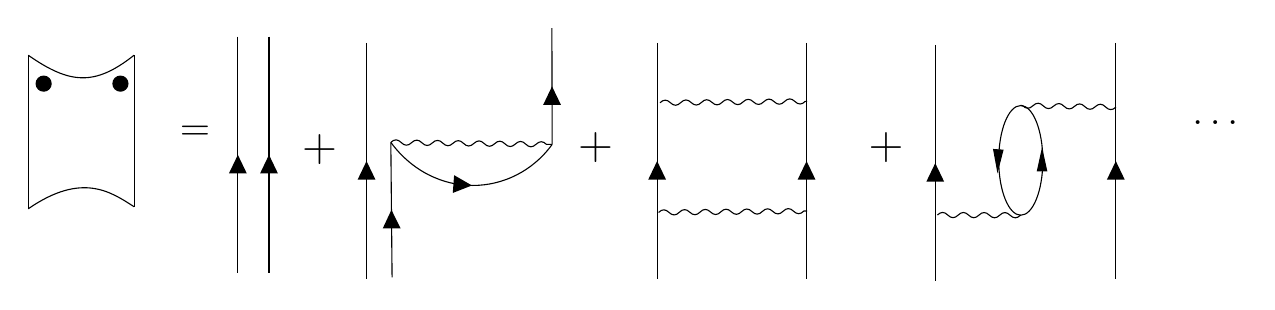
\begin{tikzpicture}[x=0.75pt,y=0.75pt,yscale=-1,xscale=1]
%uncomment if require: \path (0,300); %set diagram left start at 0, and has height of 300

%Straight Lines [id:da03751642849998316] 
\draw    (343.58,99.85) .. controls (345.23,98.17) and (346.9,98.16) .. (348.58,99.81) .. controls (350.26,101.46) and (351.93,101.44) .. (353.58,99.76) .. controls (355.23,98.08) and (356.9,98.06) .. (358.58,99.71) .. controls (360.26,101.36) and (361.93,101.34) .. (363.58,99.66) .. controls (365.23,97.98) and (366.9,97.96) .. (368.58,99.61) .. controls (370.26,101.26) and (371.93,101.24) .. (373.58,99.56) .. controls (375.23,97.88) and (376.9,97.86) .. (378.58,99.51) .. controls (380.26,101.16) and (381.93,101.14) .. (383.58,99.46) .. controls (385.23,97.78) and (386.9,97.76) .. (388.58,99.41) .. controls (390.26,101.06) and (391.93,101.04) .. (393.58,99.36) .. controls (395.23,97.68) and (396.9,97.66) .. (398.58,99.31) .. controls (400.26,100.96) and (401.92,100.94) .. (403.57,99.26) .. controls (405.22,97.58) and (406.89,97.56) .. (408.57,99.21) .. controls (410.25,100.86) and (411.92,100.84) .. (413.57,99.16) -- (414.45,99.15) -- (414.45,99.15) ;
%Straight Lines [id:da22386446930432802] 
\draw    (342.9,152.7) .. controls (344.55,151.01) and (346.22,151) .. (347.9,152.65) .. controls (349.58,154.3) and (351.25,154.28) .. (352.9,152.6) .. controls (354.55,150.92) and (356.22,150.9) .. (357.9,152.55) .. controls (359.58,154.2) and (361.25,154.18) .. (362.9,152.5) .. controls (364.55,150.82) and (366.22,150.8) .. (367.9,152.45) .. controls (369.58,154.1) and (371.25,154.08) .. (372.9,152.4) .. controls (374.55,150.72) and (376.22,150.7) .. (377.9,152.35) .. controls (379.58,154) and (381.25,153.98) .. (382.9,152.3) .. controls (384.55,150.62) and (386.22,150.61) .. (387.9,152.26) .. controls (389.58,153.91) and (391.25,153.89) .. (392.9,152.21) .. controls (394.55,150.53) and (396.22,150.51) .. (397.9,152.16) .. controls (399.58,153.81) and (401.25,153.79) .. (402.9,152.11) .. controls (404.55,150.43) and (406.22,150.41) .. (407.9,152.06) .. controls (409.58,153.71) and (411.25,153.69) .. (412.9,152.01) -- (414.52,151.99) -- (414.52,151.99) ;
%Curve Lines [id:da7645811334291478] 
\draw    (213.9,118.93) .. controls (234.62,146.93) and (272.62,145.93) .. (291.62,119.93) ;
\draw [shift={(252.97,139.68)}, rotate = 184.29] [fill={rgb, 255:red, 0; green, 0; blue, 0 }  ][line width=0.08]  [draw opacity=0] (8.93,-4.29) -- (0,0) -- (8.93,4.29) -- cycle    ;
%Straight Lines [id:da0067325630711646545] 
\draw    (213.9,118.93) -- (214.5,183.93) ;
\draw [shift={(214.2,151.43)}, rotate = 89.47] [fill={rgb, 255:red, 0; green, 0; blue, 0 }  ][line width=0.08]  [draw opacity=0] (8.93,-4.29) -- (0,0) -- (8.93,4.29) -- cycle    ;
%Straight Lines [id:da31755570766840036] 
\draw    (213.9,118.93) .. controls (215.59,117.29) and (217.25,117.31) .. (218.9,119) .. controls (220.55,120.69) and (222.21,120.71) .. (223.9,119.06) .. controls (225.59,117.42) and (227.25,117.44) .. (228.9,119.13) .. controls (230.55,120.82) and (232.21,120.84) .. (233.9,119.19) .. controls (235.59,117.54) and (237.25,117.56) .. (238.9,119.25) .. controls (240.55,120.94) and (242.21,120.96) .. (243.9,119.32) .. controls (245.59,117.67) and (247.25,117.69) .. (248.9,119.38) .. controls (250.55,121.07) and (252.21,121.09) .. (253.9,119.45) .. controls (255.59,117.8) and (257.25,117.82) .. (258.9,119.51) .. controls (260.55,121.2) and (262.21,121.22) .. (263.9,119.58) .. controls (265.59,117.93) and (267.25,117.95) .. (268.9,119.64) .. controls (270.55,121.33) and (272.21,121.35) .. (273.9,119.71) .. controls (275.59,118.06) and (277.25,118.08) .. (278.89,119.77) .. controls (280.54,121.46) and (282.2,121.48) .. (283.89,119.83) .. controls (285.58,118.19) and (287.24,118.21) .. (288.89,119.9) -- (291.62,119.93) -- (291.62,119.93) ;
%Straight Lines [id:da6864724196774904] 
\draw    (291.62,119.93) -- (291.5,63.93) ;
\draw [shift={(291.56,91.93)}, rotate = 449.88] [fill={rgb, 255:red, 0; green, 0; blue, 0 }  ][line width=0.08]  [draw opacity=0] (8.93,-4.29) -- (0,0) -- (8.93,4.29) -- cycle    ;
%Shape: Ellipse [id:dp1973299491754572] 
\draw   (517.43,154.02) .. controls (511.56,154.03) and (506.79,142.21) .. (506.77,127.62) .. controls (506.76,113.03) and (511.5,101.19) .. (517.37,101.17) .. controls (523.24,101.16) and (528.01,112.98) .. (528.03,127.57) .. controls (528.04,142.16) and (523.3,154) .. (517.43,154.02) -- cycle ;
%Straight Lines [id:da3221956834758286] 
\draw    (563.25,101.93) .. controls (561.56,103.57) and (559.89,103.54) .. (558.25,101.85) .. controls (556.61,100.16) and (554.94,100.13) .. (553.25,101.77) .. controls (551.56,103.41) and (549.89,103.38) .. (548.25,101.69) .. controls (546.61,100) and (544.94,99.97) .. (543.25,101.6) .. controls (541.56,103.24) and (539.89,103.21) .. (538.25,101.52) .. controls (536.61,99.83) and (534.94,99.8) .. (533.25,101.44) .. controls (531.56,103.07) and (529.89,103.04) .. (528.25,101.35) .. controls (526.62,99.66) and (524.95,99.63) .. (523.26,101.27) .. controls (521.57,102.91) and (519.9,102.88) .. (518.26,101.19) -- (517.37,101.17) -- (517.37,101.17) ;
%Straight Lines [id:da6584771753926739] 
\draw    (477.25,153.93) .. controls (478.92,152.27) and (480.58,152.27) .. (482.25,153.94) .. controls (483.92,155.61) and (485.58,155.61) .. (487.25,153.95) .. controls (488.92,152.29) and (490.58,152.29) .. (492.25,153.96) .. controls (493.92,155.63) and (495.58,155.63) .. (497.25,153.97) .. controls (498.92,152.31) and (500.59,152.32) .. (502.25,153.99) .. controls (503.92,155.66) and (505.58,155.66) .. (507.25,154) .. controls (508.92,152.34) and (510.58,152.34) .. (512.25,154.01) .. controls (513.92,155.68) and (515.58,155.68) .. (517.25,154.02) -- (517.43,154.02) -- (517.43,154.02) ;
%Shape: Triangle [id:dp5997188211998996] 
\draw  [fill={rgb, 255:red, 0; green, 0; blue, 0 }  ,fill opacity=1 ] (527.66,122.48) -- (529.88,132.62) -- (525.43,132.62) -- cycle ;
%Shape: Triangle [id:dp7955336974508751] 
\draw  [fill={rgb, 255:red, 0; green, 0; blue, 0 }  ,fill opacity=1 ] (506.23,132.66) -- (504.34,122.38) -- (508.79,122.68) -- cycle ;
%Straight Lines [id:da298908695859174] 
\draw    (140.2,67.93) -- (140.2,181.93) ;
\draw [shift={(140.2,124.93)}, rotate = 90] [fill={rgb, 255:red, 0; green, 0; blue, 0 }  ][line width=0.08]  [draw opacity=0] (8.93,-4.29) -- (0,0) -- (8.93,4.29) -- cycle    ;
%Straight Lines [id:da6974050351887592] 
\draw    (155.2,67.93) -- (155.2,181.93) ;
\draw [shift={(155.2,124.93)}, rotate = 90] [fill={rgb, 255:red, 0; green, 0; blue, 0 }  ][line width=0.08]  [draw opacity=0] (8.93,-4.29) -- (0,0) -- (8.93,4.29) -- cycle    ;
%Straight Lines [id:da22703180152422997] 
\draw    (202.2,70.93) -- (202.2,184.93) ;
\draw [shift={(202.2,127.93)}, rotate = 90] [fill={rgb, 255:red, 0; green, 0; blue, 0 }  ][line width=0.08]  [draw opacity=0] (8.93,-4.29) -- (0,0) -- (8.93,4.29) -- cycle    ;
%Straight Lines [id:da9259484273295726] 
\draw    (342.2,70.93) -- (342.2,184.93) ;
\draw [shift={(342.2,127.93)}, rotate = 90] [fill={rgb, 255:red, 0; green, 0; blue, 0 }  ][line width=0.08]  [draw opacity=0] (8.93,-4.29) -- (0,0) -- (8.93,4.29) -- cycle    ;
%Straight Lines [id:da9529794177037451] 
\draw    (414.2,70.93) -- (414.2,184.93) ;
\draw [shift={(414.2,127.93)}, rotate = 90] [fill={rgb, 255:red, 0; green, 0; blue, 0 }  ][line width=0.08]  [draw opacity=0] (8.93,-4.29) -- (0,0) -- (8.93,4.29) -- cycle    ;
%Straight Lines [id:da7622966924950612] 
\draw    (476.2,71.93) -- (476.2,185.93) ;
\draw [shift={(476.2,128.93)}, rotate = 90] [fill={rgb, 255:red, 0; green, 0; blue, 0 }  ][line width=0.08]  [draw opacity=0] (8.93,-4.29) -- (0,0) -- (8.93,4.29) -- cycle    ;
%Straight Lines [id:da4776407488512112] 
\draw    (563.2,70.93) -- (563.2,184.93) ;
\draw [shift={(563.2,127.93)}, rotate = 90] [fill={rgb, 255:red, 0; green, 0; blue, 0 }  ][line width=0.08]  [draw opacity=0] (8.93,-4.29) -- (0,0) -- (8.93,4.29) -- cycle    ;
%Straight Lines [id:da10037440709028045] 
\draw    (39.2,76.93) -- (39.2,150.93) ;
%Straight Lines [id:da7219080614956541] 
\draw    (90.2,76.93) -- (90.2,149.93) ;
%Curve Lines [id:da04312225103957157] 
\draw    (39.2,76.93) .. controls (59.25,90.93) and (71.25,91.93) .. (90.2,76.93) ;
%Curve Lines [id:da22574783093444029] 
\draw    (39.2,150.93) .. controls (65.25,132.93) and (79.25,142.93) .. (90.2,149.93) ;
%Shape: Circle [id:dp18876574526875] 
\draw  [fill={rgb, 255:red, 0; green, 0; blue, 0 }  ,fill opacity=1 ] (80,90.63) .. controls (80,88.62) and (81.62,87) .. (83.63,87) .. controls (85.63,87) and (87.25,88.62) .. (87.25,90.63) .. controls (87.25,92.63) and (85.63,94.25) .. (83.63,94.25) .. controls (81.62,94.25) and (80,92.63) .. (80,90.63) -- cycle ;
%Shape: Circle [id:dp7458977737708501] 
\draw  [fill={rgb, 255:red, 0; green, 0; blue, 0 }  ,fill opacity=1 ] (43,90.63) .. controls (43,88.62) and (44.62,87) .. (46.63,87) .. controls (48.63,87) and (50.25,88.62) .. (50.25,90.63) .. controls (50.25,92.63) and (48.63,94.25) .. (46.63,94.25) .. controls (44.62,94.25) and (43,92.63) .. (43,90.63) -- cycle ;

% Text Node
\draw (111,110) node [anchor=north west][inner sep=0.75pt]  [font=\Large] [align=left] {=};
% Text Node
\draw (170,114) node [anchor=north west][inner sep=0.75pt]  [font=\LARGE] [align=left] {+};
% Text Node
\draw (303,113) node [anchor=north west][inner sep=0.75pt]  [font=\LARGE] [align=left] {+};
% Text Node
\draw (443,113) node [anchor=north west][inner sep=0.75pt]  [font=\LARGE] [align=left] {+};
% Text Node
\draw (598.85,107) node [anchor=north west][inner sep=0.75pt]  [font=\Large]  {$\dotsc $};


\end{tikzpicture}

\end{center}

\subsection{No-particle amplitude (vacuum amplitude)}
\redp{The ground state energy of a many-body system may be obtained directly
from the no-particle propagator, or ' vacuum amplitude'.} This is the sum of amplitudes for all the ways the system can begin at time $t_1$ with no extra or lifted-out particles, or holes in it (this is the undisturbed or ' Fermi vacuum' state), have its particles interact with each other, and wind up at t2 with no extra or lifted-out particles, or holes. The simplest process is where nothing
at all happens-the system just sits there. A first-order process occurs in which two particles change places with each other (vacuum bubble in QFT).

\section{Classical Quasi Particles}
\subsection{The Classical Quasi Particle Propagator}
Quasi particles in a system may be tracked down by means of the single particle Green's function or 'propagator'. Let us see what this is in the classical case. Imagine we have a many-body system, and we consider the
motion of one particle in it under the influence of a constant external force $\mathbf{F}$ applied to it. Suppose the particle begins at $r_1$ at time $t_1$. If there are no collisions with other particles, the movement or 'propagation' of the particle to the point $\mathbf{r_2}$ at time $t_2$ is described by
\begin{equation}r_{2}-r_{1}=\frac{1}{2}\left(\frac{F}{m}\right)\left(t_{2}-t_{1}\right)^{2}\end{equation}
But in the interacting case, collisions take place, and the particle will follow a highly irregular path not described by the eqn. above. The best one can do in this situation is to \textbf{talk about the probability of the particle going from one point  to another.} \redp{This leads us to define the classical propagator: $P\left(\mathbf{r}_{2}, t_{2}, \mathbf{r}_{1}, t_{1}\right)$ as probability density ( = probability per unit volume) that if a particle at rest is put into the system at point $\mathbf{r}_{1}$ at time $t_{1},$ then it will be found at $\mathbf{r}_{2}$ at later time $t_{2}$.}

It will be convenient, when we later take the Fourier transform, to have $P$ defined also for $t_2<t_1$:
\begin{equation}P\left(r_{2}, t_{2}, r_{1}, t_{1}\right)=0, \text { for } t_{2}<t_{1}
\label{zero-condition}
\end{equation}
In Fig.\ref{fig:classical-quasi-particle-example} is a graph showing a qualitative picture of this propagator in the interacting and non-interacting cases. Probability density is plotted on the vertical axis, and $t_{2}$ and an arbitrary component of $\mathbf{r}_{2}$ on the horizontal axes. In the absence of interactions, $P$ will be a surface which is zero everywhere except on the line $r_{2}-r_{1}=\frac{1}{2}(F / m)\left(t_{2}-t_{1}\right)^{2},$ where it equals $\infty,$ i.e., the Dirac $\delta$-function:
\begin{equation}P_{0}\left(\mathbf{r}_{2}, t_{2}, \mathbf{r}_{1}, t_{1}\right)=\delta\left[\left(\mathbf{r}_{2}-\mathbf{r}_{1}\right)-\frac{1}{2}\left(\frac{\mathbf{F}}{m}\right)\left(t_{2}-t_{1}\right)^{2}\right]\end{equation}
\redp{This propagator in the absence of interactions is called the free propagator.}
\begin{figure}[H]
    \centering
\tikzset{every picture/.style={line width=0.75pt}} %set default line width to 0.75pt        

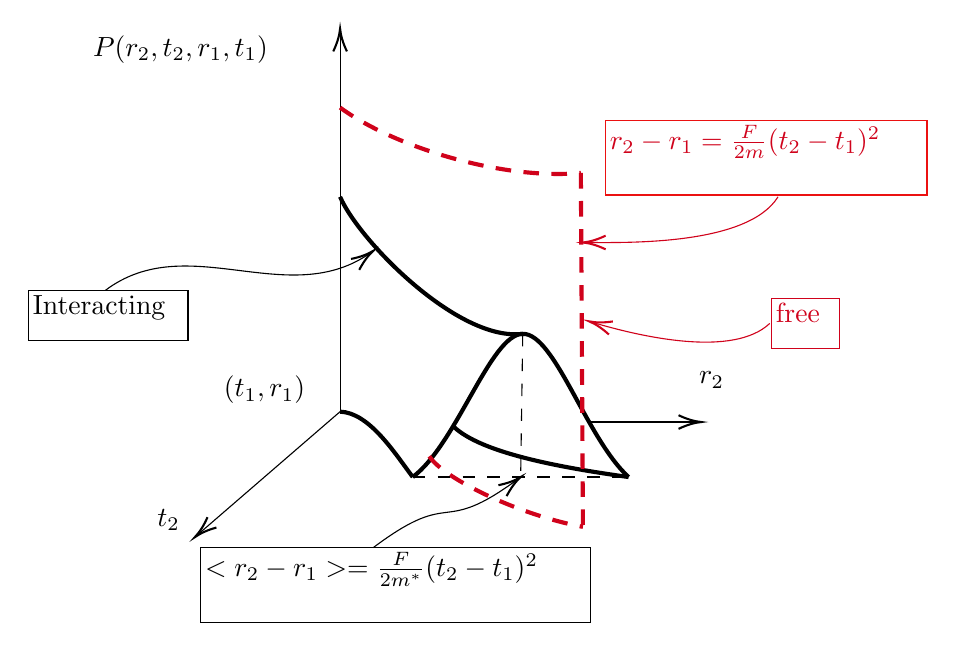
\begin{tikzpicture}[x=0.75pt,y=0.75pt,yscale=-1,xscale=1]
%uncomment if require: \path (0,300); %set diagram left start at 0, and has height of 300

%Curve Lines [id:da47195975974859194] 
\draw [line width=1.5]    (303.25,221.87) .. controls (324.47,205.95) and (340.75,153.06) .. (356.25,152.87) .. controls (371.75,152.67) and (386.71,203.02) .. (407.25,221.87) ;
%Curve Lines [id:da39634165547292277] 
\draw [line width=1.5]    (268.25,86.87) .. controls (277.25,107.87) and (325.25,156.87) .. (356.25,152.87) ;
%Straight Lines [id:da45989564554625706] 
\draw    (268.25,190.37) -- (268.25,7.87) ;
\draw [shift={(268.25,5.87)}, rotate = 450] [color={rgb, 255:red, 0; green, 0; blue, 0 }  ][line width=0.75]    (10.93,-3.29) .. controls (6.95,-1.4) and (3.31,-0.3) .. (0,0) .. controls (3.31,0.3) and (6.95,1.4) .. (10.93,3.29)   ;
%Straight Lines [id:da8675047275465586] 
\draw    (268.25,190.37) -- (199.76,249.56) ;
\draw [shift={(198.25,250.87)}, rotate = 319.15999999999997] [color={rgb, 255:red, 0; green, 0; blue, 0 }  ][line width=0.75]    (10.93,-3.29) .. controls (6.95,-1.4) and (3.31,-0.3) .. (0,0) .. controls (3.31,0.3) and (6.95,1.4) .. (10.93,3.29)   ;
%Straight Lines [id:da7098036303811813] 
\draw    (388.25,195.37) -- (440.25,195.37) ;
\draw [shift={(442.25,195.37)}, rotate = 180] [color={rgb, 255:red, 0; green, 0; blue, 0 }  ][line width=0.75]    (10.93,-3.29) .. controls (6.95,-1.4) and (3.31,-0.3) .. (0,0) .. controls (3.31,0.3) and (6.95,1.4) .. (10.93,3.29)   ;
%Curve Lines [id:da251060936963017] 
\draw [line width=1.5]    (268.25,190.37) .. controls (282.25,190.87) and (294.25,209.87) .. (303.25,221.87) ;
%Curve Lines [id:da7401245773765673] 
\draw [line width=1.5]    (323.25,197.87) .. controls (336.25,209.87) and (371.25,216.87) .. (407.25,221.87) ;
%Curve Lines [id:da4250361772641027] 
\draw [color={rgb, 255:red, 208; green, 2; blue, 27 }  ,draw opacity=1 ][line width=1.5]  [dash pattern={on 5.63pt off 4.5pt}]  (311.25,211.87) .. controls (318.25,222.87) and (355.25,240.37) .. (385.25,245.87) ;
%Straight Lines [id:da22876813296283727] 
\draw [color={rgb, 255:red, 208; green, 2; blue, 27 }  ,draw opacity=1 ][line width=1.5]  [dash pattern={on 5.63pt off 4.5pt}]  (384.25,75.37) -- (385.25,245.87) ;
%Curve Lines [id:da6869516606321976] 
\draw [color={rgb, 255:red, 208; green, 2; blue, 27 }  ,draw opacity=1 ][line width=1.5]  [dash pattern={on 5.63pt off 4.5pt}]  (268.25,43.87) .. controls (294.25,62.87) and (346.25,78.87) .. (384.25,75.37) ;
%Straight Lines [id:da7569475772419219] 
\draw  [dash pattern={on 4.5pt off 4.5pt}]  (356.25,152.87) -- (355.25,221.87) ;
%Straight Lines [id:da21545942112158833] 
\draw  [dash pattern={on 4.5pt off 4.5pt}]  (303.25,221.87) -- (407.25,221.87) ;
%Curve Lines [id:da6838743458498798] 
\draw    (284.25,255.87) .. controls (323.85,226.17) and (315.43,251.35) .. (354.06,222.75) ;
\draw [shift={(355.25,221.87)}, rotate = 503.13] [color={rgb, 255:red, 0; green, 0; blue, 0 }  ][line width=0.75]    (10.93,-3.29) .. controls (6.95,-1.4) and (3.31,-0.3) .. (0,0) .. controls (3.31,0.3) and (6.95,1.4) .. (10.93,3.29)   ;
%Curve Lines [id:da18599161011274368] 
\draw [color={rgb, 255:red, 208; green, 2; blue, 27 }  ,draw opacity=1 ]   (479.25,86.87) .. controls (464.7,110.15) and (407.81,108.96) .. (387.07,108.87) ;
\draw [shift={(385.25,108.87)}, rotate = 360] [color={rgb, 255:red, 208; green, 2; blue, 27 }  ,draw opacity=1 ][line width=0.75]    (10.93,-3.29) .. controls (6.95,-1.4) and (3.31,-0.3) .. (0,0) .. controls (3.31,0.3) and (6.95,1.4) .. (10.93,3.29)   ;
%Curve Lines [id:da8093943758486671] 
\draw    (155.25,131.87) .. controls (194.85,102.17) and (243.27,142.05) .. (283.05,113.75) ;
\draw [shift={(284.25,112.87)}, rotate = 503.13] [color={rgb, 255:red, 0; green, 0; blue, 0 }  ][line width=0.75]    (10.93,-3.29) .. controls (6.95,-1.4) and (3.31,-0.3) .. (0,0) .. controls (3.31,0.3) and (6.95,1.4) .. (10.93,3.29)   ;
%Curve Lines [id:da2739470314746484] 
\draw [color={rgb, 255:red, 208; green, 2; blue, 27 }  ,draw opacity=1 ]   (475.25,147.87) .. controls (457.7,164.44) and (413.53,154.4) .. (390.02,147.4) ;
\draw [shift={(388.25,146.87)}, rotate = 376.93] [color={rgb, 255:red, 208; green, 2; blue, 27 }  ,draw opacity=1 ][line width=0.75]    (10.93,-3.29) .. controls (6.95,-1.4) and (3.31,-0.3) .. (0,0) .. controls (3.31,0.3) and (6.95,1.4) .. (10.93,3.29)   ;

% Text Node
\draw (440,170) node [anchor=north west][inner sep=0.75pt]    {$r_{2}$};
% Text Node
\draw (179,236) node [anchor=north west][inner sep=0.75pt]    {$t_{2}$};
% Text Node
\draw (211,172) node [anchor=north west][inner sep=0.75pt]    {$( t_{1} ,r_{1})$};
% Text Node
\draw (148,8) node [anchor=north west][inner sep=0.75pt]    {$P( r_{2} ,t_{2} ,r_{1} ,t_{1})$};
% Text Node
\draw  [color={rgb, 255:red, 235; green, 17; blue, 17 }  ,draw opacity=1 ]  (396,50) -- (551,50) -- (551,86) -- (396,86) -- cycle  ;
\draw (397,51) node [anchor=north west][inner sep=0.75pt]  [color={rgb, 255:red, 208; green, 2; blue, 27 }  ,opacity=1 ]  {$r_{2} -r_{1} =\frac{F}{2m}( t_{2} -t_{1})^{2}$};
% Text Node
\draw    (201,256) -- (389,256) -- (389,292) -- (201,292) -- cycle  ;
\draw (202,257) node [anchor=north west][inner sep=0.75pt]    {$< r_{2} -r_{1}  >=\frac{F}{2m^*}( t_{2} -t_{1})^{2}$};
% Text Node
\draw    (118,132) -- (195,132) -- (195,156) -- (118,156) -- cycle  ;
\draw (119,133) node [anchor=north west][inner sep=0.75pt]   [align=left] {Interacting};
% Text Node
\draw  [color={rgb, 255:red, 208; green, 2; blue, 27 }  ,draw opacity=1 ]  (476,136) -- (509,136) -- (509,160) -- (476,160) -- cycle  ;
\draw (477,137) node [anchor=north west][inner sep=0.75pt]  [color={rgb, 255:red, 208; green, 2; blue, 27 }  ,opacity=1 ] [align=left] {free};


\end{tikzpicture}
    \caption{The classical propagator}
    \label{fig:classical-quasi-particle-example}
\end{figure}
If interactions between particles are now allowed to occur, this surface will \textbf{spread ou}t, as shown qualitatively. If we examine $\left\langle\mathbf{r}_{2}-\mathbf{r}_{1}\right\rangle,$ the position of the maximum value of $P$ in the interacting case, we see that for some types of interaction we might find that
\begin{equation}\left\langle\mathbf{r}_{2}-\mathbf{r}_{1}\right\rangle=\frac{1}{2}\left(\frac{\mathbf{F}}{m^{*}}\right)\left(t_{2}-t_{1}\right)^{2} \quad \text { for } P=\text { maximum }\end{equation}
If this is true, then \bluep{$\left\langle r_{2}-r_{1}\right\rangle$ behaves as the co-ordinate of a quasi particle of effective mass $m^{*} .$} Look now at the maximum height of $P$ as a function of $t_{2}$ Because of the 'spreading out' of the particle position, $P_{\max }$ will first fall infinitely rapidly from its value of $\infty$ at $t_{2}=t_{1},$ then more slowly. If this slower decay is exponential:
\begin{equation}P_{\max }\left(\mathbf{r}_{2}, t_{2}, \mathbf{r}_{1}, t_{1}\right) \propto e^{-\left(t_{2}-t_{1}\right) / \tau}\end{equation}
then \bluep{$\tau$ may be identified as the quasi particle lifetime;} it clearly must be fairly large if the quasi particle picture is to be useful. Thus, if we calculate $P$ and find that it shows the above behaviour, then the system is describable in terms of quasi particles and their lifetime and effective mass may be determined.

\subsection{Calculation of the Propagator by means of diagrams}
The actual calculation of the propagator P is quite complicated, but it is easy to illustrate all the principles involved with the aid of a simple analogue example in which the many-body system is replaced by \textbf{a set of fixed scattering centres}(e.g. A,B,C,D,E,F,G etc). A pinball is injected at the point $r_{1},$ at time $t_{1}$ and propagates through the system, being scattered at the various centres. We ask for the probability $P\left(\mathbf{r}_{2}, t_{2}, \mathbf{r}_{1}, t_{1}\right)$ that the particle reaches the point $r_{2}$ at time $t_{2}$.

The scattering mechanism is assumed to be such that (1) if the pinball strikes the scattering point $A$, then there is probability $P(A)$ that it is scattered and $1-P(A)$ that it will go straight through without scattering, (2) the probability distribution of pinball paths and velocities after scattering
at $A$ must be independent of the pinball path and velocity before scattering that is, the pinball loses its ' memory" of how it got to $A$.

For the sake of simplicity, let us leave time out of the argument to begin with, and consider just $P\left(\mathbf{r}_{2}, \mathbf{r}_{1}\right) ;$ this is the probability that if the particle begins at $r_{2}$ it will finish at $r_{2}$ regardless of the time. From the definition of probability, $P\left(\mathbf{r}_{2}, \mathbf{r}_{1}\right)$ is the sum of the probabilities for all the different ways the particle can go through which begin at $r_{1}$ and wind up at $r_{2}$. For example, the probability that the pinball will first hit scattering point $G$ and then end up at $r_2$ is:
\begin{equation}\left.P\left\{\left(\mathbf{r}_{1} \rightarrow \mathbf{r}_{G}\right), \text { (scattered at } \mathbf{r}_{G}\right),\left(\mathbf{r}_{G} \rightarrow \mathbf{r}_{2}\right)\right\}=P_{0}\left(\boldsymbol{r}_{G}, \mathbf{r}_{1}\right) P(G) P_{0}\left(\mathbf{r}_{2}, \mathbf{r}_{G}\right)\end{equation}
The total probability, $P\left(r_{2}, r_{1}\right),$ is just the sum of the probabilities for the various paths. Thus we find
\begin{equation}\begin{aligned}
&P\left(\mathbf{r}_{2}, \mathbf{r}_{1}\right)=P_{0}\left(\mathbf{r}_{2}, \mathbf{r}_{1}\right)+P_{0}\left(\mathbf{r}_{0}, \mathbf{r}_{1}\right) P(M) P_{0}\left(\mathbf{r}_{2}, \mathbf{r}_{0}\right)+P_{0}\left(\mathbf{r}_{M}, \mathbf{r}_{1}\right) P(M) P_{0}\left(\mathbf{r}_{2}, \mathbf{r}_{M}\right)+\\
&+P_{\mathrm{o}}\left(\mathbf{r}_{\boldsymbol{\sigma}}, \mathbf{r}_{1}\right) P(G) P_{\mathrm{o}}\left(\mathbf{r}_{\boldsymbol{G}}, \mathbf{r}_{\sigma}\right) P(G) P_{0}\left(\mathbf{r}_{2}, \mathbf{r}_{\sigma}\right)+\cdots
\end{aligned}\end{equation}
where M, and G are different scattering points.

How can this series be evaluated? If we assume that the $P_{0}$ 's are large, say $\sim \frac{1}{2}$ or so, and the various interaction $P(A)$ 's are small, say $\sim \frac{1}{10},$ then the higher order diagrams (i.e., \redp{note that by order here we mean the total number of interactions}) will give successively smaller contributions, and just as in ordinary perturbation theory, we can get an approximate solution by simply summing the series up through the first-or second-order terms. Thus, the zeroth-order approximation would be just the unperturbed case where the particle propagates freely from $\mathbf{r}_{1}$ to $\mathbf{r}_{2} .$ When we add the possibility of a perturbing (scattering) interaction with the various scattering points once each, we get the first-order approximation.

Allowing two interactions gives the second-order approximation and so on. \bluep{If, on the other hand, one or more of the interaction terms $P(A)$ is large (i.e., strong scattering at $A$ ) this method is not practical, since the series converges too slowly, and the summation must be carried out to extremely high orders to give a good result.}

However, there is another kind of approximation where we do not stop at low order interactions, but instead sums over important diagrams to infinite order. Suppose for example, that only $P(M)$ is large and all the other $P(X)$ are small. Then the "M" diagrams will dominate, and the series may be approximated by the sum over just repeated "M"s, thus:
\begin{center}
\tikzset{every picture/.style={line width=0.75pt}} %set default line width to 0.75pt        

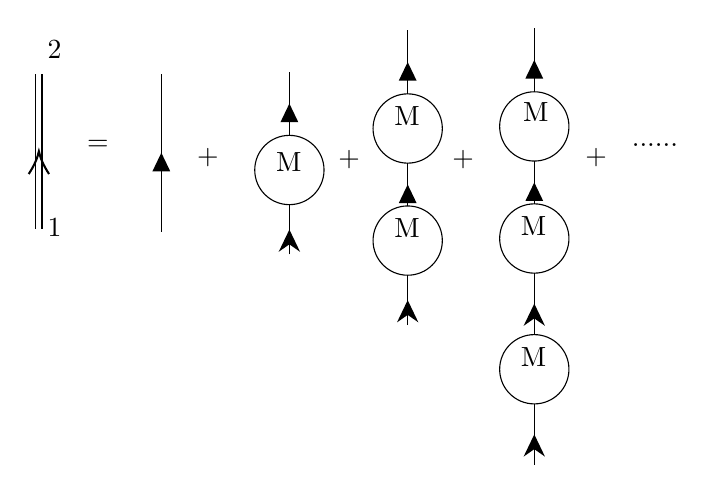
\begin{tikzpicture}[x=0.75pt,y=0.75pt,yscale=-1,xscale=1]
%uncomment if require: \path (0,349); %set diagram left start at 0, and has height of 349

%Straight Lines [id:da4757935872975344] 
\draw    (8.07,101.32) -- (8.07,26.7)(11.07,101.32) -- (11.07,26.7) ;
\draw [shift={(9.57,64.01)}, rotate = 450] [color={rgb, 255:red, 0; green, 0; blue, 0 }  ][line width=0.75]    (10.93,-4.9) .. controls (6.95,-2.3) and (3.31,-0.67) .. (0,0) .. controls (3.31,0.67) and (6.95,2.3) .. (10.93,4.9)   ;
%Straight Lines [id:da23622371172830803] 
\draw    (68.57,102.7) -- (68.57,26.7) ;
\draw [shift={(68.57,64.7)}, rotate = 450] [fill={rgb, 255:red, 0; green, 0; blue, 0 }  ][line width=0.08]  [draw opacity=0] (8.93,-4.29) -- (0,0) -- (8.93,4.29) -- cycle    ;
%Shape: Circle [id:dp4139523862436749] 
\draw   (113.57,73.01) .. controls (113.57,63.79) and (121.04,56.32) .. (130.26,56.32) .. controls (139.48,56.32) and (146.95,63.79) .. (146.95,73.01) .. controls (146.95,82.23) and (139.48,89.7) .. (130.26,89.7) .. controls (121.04,89.7) and (113.57,82.23) .. (113.57,73.01) -- cycle ;
%Straight Lines [id:da33169967910609544] 
\draw    (130.26,56.32) -- (130.26,25.7) ;
\draw [shift={(130.26,41.01)}, rotate = 450] [fill={rgb, 255:red, 0; green, 0; blue, 0 }  ][line width=0.08]  [draw opacity=0] (8.93,-4.29) -- (0,0) -- (8.93,4.29) -- cycle    ;
%Straight Lines [id:da28347419222198567] 
\draw    (130.26,113.7) -- (130.26,89.7) ;
\draw [shift={(130.26,101.7)}, rotate = 450] [fill={rgb, 255:red, 0; green, 0; blue, 0 }  ][line width=0.08]  [draw opacity=0] (10.72,-5.15) -- (0,0) -- (10.72,5.15) -- (7.12,0) -- cycle    ;
%Shape: Circle [id:dp663325870350397] 
\draw   (170.57,107.01) .. controls (170.57,97.79) and (178.04,90.32) .. (187.26,90.32) .. controls (196.48,90.32) and (203.95,97.79) .. (203.95,107.01) .. controls (203.95,116.23) and (196.48,123.7) .. (187.26,123.7) .. controls (178.04,123.7) and (170.57,116.23) .. (170.57,107.01) -- cycle ;
%Straight Lines [id:da6913773132395338] 
\draw    (187.26,36.32) -- (187.26,5.7) ;
\draw [shift={(187.26,21.01)}, rotate = 450] [fill={rgb, 255:red, 0; green, 0; blue, 0 }  ][line width=0.08]  [draw opacity=0] (8.93,-4.29) -- (0,0) -- (8.93,4.29) -- cycle    ;
%Straight Lines [id:da4724377841227787] 
\draw    (187.26,147.7) -- (187.26,123.7) ;
\draw [shift={(187.26,135.7)}, rotate = 450] [fill={rgb, 255:red, 0; green, 0; blue, 0 }  ][line width=0.08]  [draw opacity=0] (10.72,-5.15) -- (0,0) -- (10.72,5.15) -- (7.12,0) -- cycle    ;
%Shape: Circle [id:dp29262051024858293] 
\draw   (170.57,53.01) .. controls (170.57,43.79) and (178.04,36.32) .. (187.26,36.32) .. controls (196.48,36.32) and (203.95,43.79) .. (203.95,53.01) .. controls (203.95,62.23) and (196.48,69.7) .. (187.26,69.7) .. controls (178.04,69.7) and (170.57,62.23) .. (170.57,53.01) -- cycle ;
%Straight Lines [id:da2293551017015375] 
\draw    (187.26,69.7) -- (187.26,90.32) ;
\draw [shift={(187.26,80.01)}, rotate = 90] [fill={rgb, 255:red, 0; green, 0; blue, 0 }  ][line width=0.08]  [draw opacity=0] (8.93,-4.29) -- (0,0) -- (8.93,4.29) -- cycle    ;
%Shape: Circle [id:dp5742274191772756] 
\draw   (231.57,106.01) .. controls (231.57,96.79) and (239.04,89.32) .. (248.26,89.32) .. controls (257.48,89.32) and (264.95,96.79) .. (264.95,106.01) .. controls (264.95,115.23) and (257.48,122.7) .. (248.26,122.7) .. controls (239.04,122.7) and (231.57,115.23) .. (231.57,106.01) -- cycle ;
%Straight Lines [id:da8337372469854066] 
\draw    (248.26,35.32) -- (248.26,4.7) ;
\draw [shift={(248.26,20.01)}, rotate = 450] [fill={rgb, 255:red, 0; green, 0; blue, 0 }  ][line width=0.08]  [draw opacity=0] (8.93,-4.29) -- (0,0) -- (8.93,4.29) -- cycle    ;
%Straight Lines [id:da42712440571211296] 
\draw    (248.26,152.07) -- (248.26,122.7) ;
\draw [shift={(248.26,137.38)}, rotate = 450] [fill={rgb, 255:red, 0; green, 0; blue, 0 }  ][line width=0.08]  [draw opacity=0] (10.72,-5.15) -- (0,0) -- (10.72,5.15) -- (7.12,0) -- cycle    ;
%Shape: Circle [id:dp5287893719741432] 
\draw   (231.57,52.01) .. controls (231.57,42.79) and (239.04,35.32) .. (248.26,35.32) .. controls (257.48,35.32) and (264.95,42.79) .. (264.95,52.01) .. controls (264.95,61.23) and (257.48,68.7) .. (248.26,68.7) .. controls (239.04,68.7) and (231.57,61.23) .. (231.57,52.01) -- cycle ;
%Straight Lines [id:da8377025286119076] 
\draw    (248.26,68.7) -- (248.26,89.32) ;
\draw [shift={(248.26,79.01)}, rotate = 90] [fill={rgb, 255:red, 0; green, 0; blue, 0 }  ][line width=0.08]  [draw opacity=0] (8.93,-4.29) -- (0,0) -- (8.93,4.29) -- cycle    ;
%Shape: Circle [id:dp8985140189745163] 
\draw   (231.57,169.01) .. controls (231.57,159.79) and (239.04,152.32) .. (248.26,152.32) .. controls (257.48,152.32) and (264.95,159.79) .. (264.95,169.01) .. controls (264.95,178.23) and (257.48,185.7) .. (248.26,185.7) .. controls (239.04,185.7) and (231.57,178.23) .. (231.57,169.01) -- cycle ;
%Straight Lines [id:da5985992460409527] 
\draw    (248.26,215.07) -- (248.26,185.7) ;
\draw [shift={(248.26,200.38)}, rotate = 450] [fill={rgb, 255:red, 0; green, 0; blue, 0 }  ][line width=0.08]  [draw opacity=0] (10.72,-5.15) -- (0,0) -- (10.72,5.15) -- (7.12,0) -- cycle    ;

% Text Node
\draw (12.57,95.32) node [anchor=north west][inner sep=0.75pt]   [align=left] {1};
% Text Node
\draw (12.57,9.32) node [anchor=north west][inner sep=0.75pt]   [align=left] {2};
% Text Node
\draw (31.57,57.32) node [anchor=north west][inner sep=0.75pt]   [align=left] {=};
% Text Node
\draw (122.57,63.32) node [anchor=north west][inner sep=0.75pt]   [align=left] {M};
% Text Node
\draw (241.57,39.32) node [anchor=north west][inner sep=0.75pt]   [align=left] {M};
% Text Node
\draw (240.57,94.32) node [anchor=north west][inner sep=0.75pt]   [align=left] {M};
% Text Node
\draw (179.57,95.32) node [anchor=north west][inner sep=0.75pt]   [align=left] {M};
% Text Node
\draw (179.57,41.32) node [anchor=north west][inner sep=0.75pt]   [align=left] {M};
% Text Node
\draw (84.57,61.32) node [anchor=north west][inner sep=0.75pt]    {$+$};
% Text Node
\draw (152.57,62.32) node [anchor=north west][inner sep=0.75pt]    {$+$};
% Text Node
\draw (207.57,62.32) node [anchor=north west][inner sep=0.75pt]    {$+$};
% Text Node
\draw (271.57,61.32) node [anchor=north west][inner sep=0.75pt]    {$+$};
% Text Node
\draw (240.57,157.32) node [anchor=north west][inner sep=0.75pt]   [align=left] {M};
% Text Node
\draw (294,59) node [anchor=north west][inner sep=0.75pt]   [align=left] {......};


\end{tikzpicture}

\end{center}
Translating each element of the diagrams into the appropriate probability, it is easy to write down the corresponding series:
$$\begin{aligned}
P\left(\mathbf{r}_{2}, \mathbf{r}_{1}\right) \approx P_{0} &\left(\mathbf{r}_{2}, \mathbf{r}_{1}\right)+P_{0}\left(\mathbf{r}_{\mathbf{M}}, \mathbf{r}_{1}\right) P(M) P_{0}\left(\mathbf{r}_{2}, \mathbf{r}_{M}\right)+\\
&+P_{0}\left(\mathbf{r}_{M}, \mathbf{r}_{1}\right) P(M) P_{0}\left(\mathbf{r}_{M}, \mathbf{r}_{M}\right) P(M) P_{0}\left(\mathbf{r}_{2}, \mathbf{r}_{M}\right)+\cdots
\end{aligned}$$
and
$$\begin{aligned}
P\left(\mathbf{r}_{2}, \mathbf{r}_{1}\right) \approx P_{0}\left(\mathbf{r}_{2}, \mathbf{r}_{1}\right)+P_{0}\left(\mathbf{r}_{M}, \mathbf{r}_{1}\right) P(M) P_{0}\left(\mathbf{r}_{2}, \mathbf{r}_{M}\right) \times & \\
\times\left[1+P(M) P_{0}\left(\mathbf{r}_{M}, \mathbf{r}_{M}\right)+P(M)^{2} P_{0}\left(\mathbf{r}_{M}, \mathbf{r}_{M}\right)^{2}+\cdots\right] \\
=P_{0}\left(\mathbf{r}_{2}, \mathbf{r}_{1}\right)+\frac{P_{0}\left(\mathbf{r}_{M}, \mathbf{r}_{1}\right) P(M) P_{0}\left(\mathbf{r}_{2}, \mathbf{r}_{M}\right)}{1-P(M) P_{0}\left(\mathbf{r}_{M}, \mathbf{r}_{M}\right)}
\end{aligned}$$
This new approximation, involving the summation of a perturbation series to infinite order over a selected class of repeated diagrams (i.e., terms) is called' partial summation' or' selective summation'. It is drastically different from the ordinary perturbation approximation.

The above diagram technique may easily be extended to the time-dependent propagator, $P\left(\mathbf{r}_{2}, \mathbf{r}_{1}, t_{2}-t_{1}\right) .$ (We have written $t_{2}-t_{1}$ since the force is time independent so the propagators can depend only on time differences.) Let $P_{0}\left(\mathbf{r}_{j}, \mathbf{r}_{i}, t_{j}-t_{i}\right)=$ probability that if the particle leaves the point $\mathbf{r}_{i}$ at time $t_{i}$ then it arrives at $r_{j}$ at time $t_{j}$ without undergoing any interaction on the way (this is the 'free propagator'). Let $P(A)$ be the interaction term, assumed instantaneous for simplicity. Then, we have
\begin{equation}\begin{aligned}
P\left(\mathbf{r}_{2}, \mathbf{r}_{1}, t_{2}-t_{1}\right)=& P_{0}\left(\mathbf{r}_{2}, \mathbf{r}_{1}, t_{2}-t_{1}\right)+\\
&+\int_{t_{1}}^{t_{2}} d t_{G} P_{0}\left(\mathbf{r}_{G}, \mathbf{r}_{1}, t_{G}-t_{1}\right) P(G) P_{0}\left(\mathbf{r}_{2}, \mathbf{r}_{G}, t_{2}-t_{G}\right)+\\
&+\int d t_{M} \cdots+\iint+\cdots+\iiint+\cdots+\cdots
\end{aligned}
\label{pinball-example}
\end{equation}
The integrals parading through this expansion can be removed by noticing that they all have the form of "folded" products. This means they can be converted into simple products by a Fourier transformation. Suppose we define the transformed propagator, $P_0(\mathbf{r}_j,\mathbf{r}_i,\omega)$ by
\begin{equation}P_{0}\left(\mathbf{r}_{j}, \mathbf{r}_{i}, t_{j}-t_{l}\right)=\frac{1}{2 \pi} \int_{-\infty}^{+\infty} d \omega e^{-i \omega\left(t_{j}-t_i\right)} P_{0}\left(\mathbf{r}_{j}, \mathbf{r}_{i}, \omega\right)\end{equation}
with a similar expression for $P\left(\mathbf{r}_{j}, \mathbf{r}_{l}, \omega\right) .$ Then the first two terms of (\ref{pinball-example}) become (note that we can integrate over $t_{G}$ from $-\infty$ to $+\infty$ because condition
(\ref{zero-condition}) automatically limits the integral to the region $t_{1} \rightarrow t_{2}$ ):
$$P_{0}\left(\mathbf{r}_{2}, \mathbf{r}_{1}, t_{2}-t_{1}\right)=\frac{1}{2 \pi} \int_{-\infty}^{+\infty} d \omega e^{-i \omega\left(t_{2}-t_{1}\right)} P_{0}\left(\mathbf{r}_{2}, \mathbf{r}_{1}, \omega\right)$$
$$\begin{array}{l}
\int_{-\infty}^{+\infty} d t_{G} P_{0}\left(\mathbf{r}_{G}, \mathbf{r}_{1}, t_{G}-t_{1}\right) P(G) P_{0}\left(\mathbf{r}_{2}, \mathbf{r}_{G}, t_{2}-t_{G}\right)= \\
=\int_{-\infty}^{+\infty} d t_{G}\left[\frac{1}{2 \pi} \int_{-\infty}^{+\infty} d \omega^{\prime} e^{-i \omega^{\prime}\left(t_{G}-t\right)} P_{0}\left(\mathbf{r}_{G}, \mathbf{r}_{1}, \omega^{\prime}\right)\right] \times \\
\quad \times P(G) \times\left[\frac{1}{2 \pi} \int_{-\infty}^{+\infty} d \omega e^{-i \omega\left(t_{2}-t_{G}\right)} P_{0}\left(\mathbf{r}_{2}, \mathbf{r}_{G}, \omega\right)\right]=
\end{array}$$
$$\begin{array}{c}
=\frac{1}{(2 \pi)^{2}} \int_{-\infty}^{+\infty} d \omega \int_{-\infty}^{+\infty} d \omega^{\prime} P_{0}\left(\mathbf{r}_{G}, \mathbf{r}_{1}, \omega^{\prime}\right) \times \\
\times P(G) P_{0}\left(\mathbf{r}_{2}, \mathbf{r}_{G}, \omega\right) e^{+i\left(\omega^{\prime} t_{1}-\omega t_{2}\right)} \int_{-\infty}^{+\infty} d t_{G} e^{-i t_{0}\left(\omega^{\prime}-\omega\right)}
\end{array}$$
Since
\begin{imp}
\begin{equation}
2 \pi \delta\left(\omega^{\prime}-\omega\right)=\int_{-\infty}^{+\infty} d t_{G} e^{-i t_{G}\left(\omega^{\prime}-\omega\right)}\end{equation}
\end{imp}
we have
\begin{equation}
\begin{aligned}
\int_{-\infty}^{+\infty} d t_{G} P_{0}\left(\mathbf{r}_{G}, \mathbf{r}_{1}, t_{G}-t_{1}\right) P(G) P_{0}\left(\mathbf{r}_{2}, \mathbf{r}_{G}, t_{2}-t_{G}\right)&=\\
&\frac{1}{2 \pi} \int_{-\infty}^{+\infty} d \omega e^{-i \omega\left(t_{2}-t_{1}\right)} P_{0}\left(\mathbf{r}_{G}, \mathbf{r}_{1}, \omega\right) P(G) P_{0}\left(\mathbf{r}_{2}, \mathbf{r}_{G}, \omega\right)
\end{aligned}
\end{equation}
Continuing thus, and finally taking the inverse transform, yields
\begin{equation}P\left(\mathbf{r}_{2}, \mathbf{r}_{1}, \omega\right)=P_{0}\left(\mathbf{r}_{2}, \mathbf{r}_{1}, \omega\right)+P_{0}\left(\mathbf{r}_{G}, \mathbf{r}_{1}, \omega\right) P(G) P_{0}\left(\mathbf{r}_{2}, \mathbf{r}_{G}, \omega\right)+\cdots\end{equation}

\section{Quantum Quasi Particles and the Quantum Pinball Propagator}
In the quantum case, the total probability amplitude is the sum of the probability amplitudes for each process taken separately
$$G(2,1)=G(\text { process } 1)+G(\text { process } 11)+\cdots$$
so that the corresponding probability is given by
$$P(2,1)_{\text {quantum }}=G^{*} G=\underbrace{|G(\mathrm{I})|^{2}}_{P(\mathrm{I})}+\underbrace{|G(\mathrm{I})|^{2}}_{P(\mathrm{II})}+\underbrace{G(\mathrm{I})^{*} G(\mathrm{II})+G(\mathrm{II})^{*} G(\mathrm{I})}_{\text {interference terms }}+\cdots$$
Because of the characteristic interference terms', the quantum probability is not just the sum of the probabilities for the individual processes, in contrast to the classical case.

Let us begin by defining the quantum propagator in general, then show
what it looks like in the case of free particles and quasi particles. The quantum analogue of the classical propagator is (assuming that the Hamiltonian is time-independent, so that the propagator depends only on time differences):
\begin{imp}
\begin{equation}i G\left(\mathrm{r}_{2}, \mathrm{r}_{1}, t_{2}-t_{1}\right)_{t_{2}>t_{1}}=i G^{+}\left(\mathrm{x}_{2}, \mathrm{r}_{1}, t_{2}-t_{1}\right)\end{equation}
probability amplitude that if at time $t_{1}$ we add a particle at point $r_{1}$ to the interacting system in its ground state, then at time $t_{2}$ the system will be in its ground state with an added particle at $\mathbf{r}_{2}$
\end{imp}
The $i$ factor is purely for decoration (a matter of convention) and the $+$ superscript denotes $t_{2}>t_{1} .$ The probability corresponding to the amplitude is
$$P\left(\mathbf{r}_{2}, \mathbf{r}_{1}, t_{2}-t_{1}\right)=G^{+}\left(r_{2}, \mathbf{r}_{1}, t_{2}-t_{1}\right)^{*} G^{+}\left(\mathbf{r}_{2}, \mathbf{r}_{1}, t_{2}-t_{1}\right)$$
Note that it is not necessarily the 'same' particle which is observed at 12, since
this has no meaning in the systems of identical particles with which we shall generally deal. The quantity $G^{+}$ is called a \bluep{'retarded' propagator (or Green's function)}. By definition, it is equal to zero for $t_{2} \leqslant t_{1} .$ There is also an \bluep{'advanced' propagator, $G^{-},$ which is finite for $t_{2} \leqslant t_{1} $}.

It is actually more convenient to work with an equivalent definition of $G$ in terms of arbitrary single-particle eigenstates, $\phi_{k}(r),$ instead of position eigenstates. Then we have \redp{$i G^{+}\left(k_{2}, k_{1}, t_{2}-t_{1}\right)_{t_{2}>t_{1}}=$probability amplitude that if at time $t_{1}$ we add a particle in $\phi_{k_{1}}(r)$ to the interacting system in its ground state, then at time $t_{2}$ the system will be in its ground state with an added particle in $\phi_{k_{2}}(r)$}.
For $t_{2} \leqslant t_{1}, G^{+}$ is defined so that:
\begin{equation}i G^{+}\left(k_{2}, k_{1}, t_{2}-t_{1}\right)_{t_{2}\leq t_{1}}=0\end{equation}
\textbf{A convenient choice for $\phi_{k}(r)$ is the eigenstates of the unperturbed single particle Hamiltonian, which we will call $H_{0}$ :}
$$H_{0}=\frac{p^{2}}{2 m}+U(\mathrm{r})=-\frac{1}{2 m} \nabla_{r}^{2}+U(\mathrm{r}) \quad(\hbar=1)$$
If $U(\mathrm{r})=0,$ then this is just the free particle case:
$$H_{0} \phi_{k}(\mathbf{r})=\epsilon_{k} \phi_{k}(\mathbf{r})$$
and
\begin{equation}H_{0}=-\frac{\nabla_{r}^{2}}{2 m}, \quad \phi_{k}(r)=\frac{1}{\sqrt{\Omega}} e^{i k \cdot r}, \quad \epsilon_{k}=\frac{k^{2}}{2 m}
\label{nrqm-free-particle}
\end{equation}
where $\Omega$ is normalization volume and spin is neglected for simplicity. Note that if $k_1=k_2$, the particle propagates in time only.

Let us first get the free propagator $G_{0}^{+}$ (no perturbing interaction). Suppose at time $t_{1}$ the wave function of the free particle is $\phi_{k,}(\mathrm{r}) .$ Then we have:
$$\psi\left(\mathbf{r}, t_{1}\right)=\phi_{\mathbf{k}_{2}}(\mathbf{r})$$
At later time $t_{2},$ by the time-dependent Schrödinger equation, we find that the wave function has become
\begin{equation}\psi\left(\mathbf{r}, t_{2}\right)=\phi_{k_{1}}(\mathbf{r}) e^{-i \varepsilon_{k1}\left(t_{2}-t_{1}\right)}
\end{equation}
where $\epsilon_{k_{1}}$ is the single particle energy of undisturbed Shrodinger equation. The probability amplitude for the particle being in state $\phi_{k_{2}}$ at time $t_{2}$ is /hen just the component of $\psi\left(\mathbf{r}, t_{2}\right)$ along $\phi_{k_{2}}$ or:
\begin{equation}\int d^{3} \mathbf{r} \psi\left(\mathbf{r}, t_{2}\right) \phi_{k_{2}}^{*}(\mathbf{r})=e^{-i \exp \left(l_{2}-t_{1}\right)} \int \underbrace{d^{3} \mathbf{r} \phi_{k_{1}}(\mathbf{r}) \phi_{k_{2}}^{*}(\mathbf{r})}_{\delta_{k_{2} k_{1}}}\end{equation}
whence, by definition
\begin{equation}G_{0}^{+}\left(k, t_{2}-t_{1}\right)=\left\{\begin{array}{ll}
-i \theta_{12-t_{1}} e^{-i \epsilon_{k_1}\left(t_{2}-t_{1}\right)}, & \text { for } t_{2} \neq t_{1} \\
0, & \text { for } t_{2}=t_{1}
\end{array}\right.
\label{G0-+}
\end{equation}
where
$$\theta_{t_{2}-t_{1}}\left\{\begin{array}{ll}
=1, & \text { if } t_{2}>t_{1} \\
=0, & \text { if } t_{2}<t_{1}
\end{array}\right.$$
\bluep{Note that for fermions, all levles up to $\epsilon_F$(=Fermi energy) are fileed, so we can only propagate a particle with $\epsilon_{k_1}>\epsilon_F$}. The Fourier transform of (\ref{G0-+}) is
\begin{equation}\begin{aligned}
G_{0}^{+}(k, \omega) &=-i \int_{-\infty}^{+\infty} d\left(t_{2}-t_{1}\right) \theta_{t_{2}-t_{1}} e^{i \omega\left(t_{2}-t_{1}\right)} e^{-i \epsilon_{k}\left(t_{2}-t_{1}\right)} \\
&=\left.(-1) \frac{e^{i\left(\omega-\epsilon_{k}\right)\left(t_{2}-t_{1}\right)}}{\omega-\epsilon_{k}}\right|_{0} ^{\infty}=\frac{1}{\omega-\epsilon_{k}}-\frac{e^{i\left(\omega-\epsilon_{k}\right)\infty}}{\omega-\epsilon_{k}}
\end{aligned}
\label{G0-k-omega}
\end{equation}
\redp{Because of the exponential oscillating at $\infty,$ this function is not well defined. In order to get around this difficulty, we have to slightly modify the expression for the free propagator. This is done by multiplying the propagator by the factor $\exp \left(-\delta\left(t_{2}-t_{1}\right)\right),$ where $\delta$ is a positive infinitesimal such that $\delta \times \infty=\infty$}. Then (\ref{G0-+}) becomes:
\begin{equation}G_{0}^{+}\left(k, t_{2}-t_{1}\right)=-i \theta_{t_{2}-t_{1}}e^{i(\epsilon_k-i\delta)(t_2-t_1)}
\label{G0-with-delta}
\end{equation}
For any finite $\left(t_{2}-t_{1}\right),$ we have $\delta \times\left(t_{2}-t_{1}\right)=0,$ so this is just $(3.10) .$ But for infinite $\left(t_{2}-t_{1}\right), \delta \times\left(t_{2}-t_{1}\right)=\infty$ so $G_{0}^{+}=0 .$ When \ref{G0-with-delta} is placed in \ref{G0-k-omega} we find
\begin{imp}
\begin{equation}G_{o}^{+}(k, \omega)=\frac{1}{\omega-\epsilon_{k}+i \delta}
\label{G0-k-omega-delta}
\end{equation}
\end{imp}
\bluep{From \ref{G0-k-omega-delta} we see the pole is at $\omega=\epsilon_k$, the eigenvalue for the eigenstate $\phi_k$. It turns out this observation is quite general, even for interacting propagator, $G^0(k,l;\omega)$:}
\begin{imp}
The poles of $G^+(k,l,\omega),$ the fourier transform of the single-particle propagator, corresponds to the excited energy of (N+1)-particle system \textbf{minus the ground state energy of N-particle system}.
\end{imp}
Also from \ref{G0-k-omega-delta}, we have the particle lifetime $\tau$ as $\delta^{-1}=\infty$, which makes sense because we only consider one free particle here. This observation can also be extended to interacting system where the propagator has the form of 
\begin{equation}
    G^+=\frac{1}{\omega-\epsilon_k^{\prime}+i\tau_k^{-1}}
\end{equation}
where \redp{$\tau_k$ is the quasi-particle lifetime at the state of $\epsilon_k$}.

In a Fermi system, because of the Pauli's principle, each state can only be occupied by one fermion. If a state is partially occupied by a fermion, the possibility of adding another fermion at the same state will be less than 1. Hence we have to multiply the propagator by a factor $Z_k\leq 1$:
\begin{equation}G_{\text {\stackanchor{quasi}{particle} }}^{+}\left(k,t_{2}-t_{1}\right)=-i Z_{k} e^{-i \epsilon_{k}^{\prime}\left(t_{2}-t_{1}\right)} e^{-\left(t_{2}-t_{1}\right) / \tau_{k}}\end{equation}
\begin{equation}G_{\text {\stackanchor{quasi}{particle}}}^{+}(k, \omega)=\frac{Z_{k}}{\omega-\epsilon_{k}^{\prime}+i \tau_{k}^{-1}}\end{equation}
The poles in the equation above are 
\begin{equation}
    \omega = \epsilon_k^{\prime}-i\tau_k^{-1}
\end{equation}
We can still interpret these poles as the excited energy levels even though they are imaginary numbers. For free particles, we have eigenstates as:
$$
\psi_k(x)=\phi_k(x)e^{-i\epsilon_k t}
$$
When the weak interaction is turned on, the particle decays out of state "$k$", we have
$$
\psi_k(x)\approx\phi_k(x)e^{-i\epsilon_k^{\prime} t}e^{-t/\tau_k}=\phi_k(x)e^{-i(\epsilon_k^{\prime}-i\tau^{-1})t}
$$

\subsection{Quantum Pinball Game}
Like the classical pinball game, we now consider the quantum version of the game where \redp{the "scattering centers" are now "scattering fields/potentials"}. Let's assume that a perturbative potential that interacts with free particle has a form of:
\begin{equation}V(\mathbf{p})=V_{M}+V_{L}=M p^{2}+L p^{4}=-M \nabla_{r}^{2}+L \nabla_{r}^{4}\end{equation}
where $M \geqslant L$. By solving the Schrodinger equation we have the Hamiltonian as
$$
H = (\frac{1}{2m}+M+Lp^2)p^2
$$
with 
$$
\epsilon_k^{\prime}= (\frac{1}{2m}+M+Lk^2)k^2
$$
and $\phi_k(x)=\frac{1}{\sqrt{\Omega}}e^{-i\mathbf{k}\cdot\mathbf{r}}$.\bluep{Now let us solve for the eigenvalues in a propagator way.}

The simplest way the particle can propagate through the system is without interaction, which has a propability amplitude as $G^+(k,t_2-t_1)$. Another way is to enter in $\phi_{k_{1}}$ at time $t_{1},$ be scattered into state $\phi_{k_{2}}$ at time $t_{M}$ by the potential $V_{M},$ then continue freely in $\phi_{k_{2}}$ until time $t_{2} .$ The probability amplitude in this case is just the product of the probability amplitude for each independent process:
$$
G^+_0(k_1,t_M-t_1)V_MG^+_0(k_1,t_2-t_M)
$$
$V_M$ can be obtained from time-dependent perturbation theory as follows: Let $c_{l}$ be the probability amplitude that at time $t_{0}$ a system is in state $\phi_{l} .$ Then at later time, $t,$ the time rate of change of any particular $c_{l},$ say $c_{p},$ under the influence of perturbation $V$, is given by:
\begin{equation}\dot{c}_{p}(t)=-i \sum_{l} V_{p l} c_{l} e^{i\left(\epsilon_{p}-c_{l}\right)\left(t-t_{o}\right)}\end{equation}
where $V_{pl}$ is just the element of S matrix. Hence the probability amplitude per unit time that the system undergoes a transition from $\phi_{k_1}$ to $\phi_p=\phi_{k_2}$, at time $t_M$ is:
\begin{equation}\begin{aligned}
\dot{c}_{k_{2}}\left(t=t_{M}\right) &=-i V_{M_{k_2 k_1}}=-i \int d^{3} \mathbf{r} \phi_{k_{2}}^{*}(r) V_{M} \phi_{k_{1}}(r)=\\
&=+i M \int d^{3} \mathbf{r} \phi_{k_{2}}^{*} \nabla^{2} \phi_{k_{1}}=-i M k_{1}^{2} \delta_{k_{2} k_{1}}
\end{aligned}\end{equation}
Thus the probability amplitude for this first-order scattering is 
\begin{equation}
    \left[\text{\stackanchor{probability}{amplitude}}\right]_{t_1\rightarrow t_M\rightarrow t_2}=i \int_{-\infty}^{+\infty} d t_{M} G_{0}^{+}\left(\mathbf{k}_{1}, t_{M}-t_{1}\right) V_{M_{k_2k_1}} G_{0}^{+}\left(\mathbf{k}_{2}, t_{2}-t_{M}\right)
\end{equation}
Similarly for $V_L$, we have
$$-i V_{L_{k_1k_2}}=-i L k_{1}^{4} \delta_{k_{2} k_{1}}$$
which also conserves momentum. There are also second- and higher-order processes in which the particle collides with $V_{M}$ and $V_{L}$ any number of times. This gives us the series expansion for the propagator (set $\mathbf{k}_{1}=\mathbf{k}_{2}=\mathbf{k}$ because of conservation of momentum here), after cancelling the $i$ 's:
$$\begin{aligned}
G^{+}\left(\mathbf{k}, t_{2}-t_{1}\right)=G_{0}^{+} &\left(\mathbf{k}, t_{2}-t_{1}\right)+\int_{-\infty}^{+\infty} d t_{M} G_{0}^{+}\left(\mathbf{k}, t_{M}-t_{1}\right) V_{M} G_{0}^{+}\left(\mathbf{k}, t_{2}-t_{M}\right) \\
&+\int_{-\infty}^{+\infty} d t_{L} G_{0}^{+}\left(\mathbf{k}, t_{L}-t_{1}\right) V_{L} G_{0}^{+}\left(\mathbf{k}, t_{2}-t_{L}\right)+\\
&+\int d t_{M} d t_{M}^{\prime} \cdots+\int d t_{M} d t_{L} \cdots+\cdots
\end{aligned}$$
Taking the Fourier transform, we have
\begin{equation}\begin{aligned}
G^{+}(\mathbf{k}, \omega)=G_{0}^{+} &(\mathbf{k}, \omega)+\left[G_{0}^{+}(\mathbf{k}, \omega)\right]^{2} V_{M_{k k}}+\left[G_{0}^{+}(\mathbf{k}, \omega)\right]^{2} V_{L_{kk}}+\\
&+\left[G_{0}^{+}\right]^{3} V_{M_{kk}}^{2}+2\left[G_{0}^{+}\right]^{3} V_{M_{kk}} V_{L_{kk}}+\left[G_{0}^{+}\right]^{3} V_{L_{kk}}^{2}+\\
&+\left[G_{0}^{+}\right]^{4} V_{M_{kk}}^{3}+\cdots
\end{aligned}\end{equation}
We now pull the trick of \redp{partial summation} here. We assume that the scattering with $V_M$ is much more important than the scattering with $V_L$, then the Feynman diagram series can be approximated by:



\end{document}